\documentclass[fleqn, 12pt]{article}

\usepackage[utf8]{inputenc}
\usepackage[bulgarian]{babel}
\usepackage{amsmath}
\usepackage{amssymb}
\usepackage{booktabs}
\usepackage{fancyhdr}
\usepackage{amsthm}
\usepackage{tikz}
\usepackage{centernot}

\theoremstyle{definition}
\newtheorem{example}{Пример}[subsection]
\newtheorem{definition}{Дефиниция}[subsection]
\newtheorem{axiom}{Аксиома}[subsection]
\newtheorem{theorem}{Теорема}[subsection]
\newtheorem{lemma}{Лема}[subsection]

\title{Дискретна математика}
\author{Exonaut}

\pagestyle{fancy}
\fancyhf{}
\lhead{\rightmark}
\rhead{\thepage}
\cfoot{}
\renewcommand{\headrulewidth}{0pt}

\begin{document}
\maketitle
\pagenumbering{gobble}

\newpage
\pagenumbering{arabic}

\tableofcontents
\newpage

\section{Лекция 1: Логика и логически оператори}

\subsection{Дефиниции}

\begin{definition}
\textbf{Логиката} е система, базирана на съждения
\end{definition}

\begin{definition}
\textbf{Съждението} е твърдение което може да бъде истина или лъжа (но не и двете едновеременно).\\
Следователно резултатът от едно съждение може да бъде истина(И) или ако то е вярно или лъжа (Л), ако е грешно.
\end{definition}

\begin{definition}
Съжденията, които не съдържат в себе си други съждения, се наричат \textbf{прости}.
\end{definition}

\begin{definition}
Едно и няколко съждения могат да бъдат обединени в едно единствено \textbf{комбинирано съждение}, посредством логически оператори. 
\end{definition}

\begin{definition}
\textbf{Таблица на истинност} се нарича таблица, в която се изброяват всички възможни комбинации от стойности  на отделните променливи в съждението, както и съответните стойности на функцията. 
\end{definition}

\begin{definition}
Две \textbf{съждения са еквиваленти}, ако имат една и съща таблица на истинност или следват едно от друго вследствие прилагани основни закони за преобразуване. 
\end{definition}
\newpage
\subsection{Логически оператори}

\subsubsection{Отрицание(NOT)}
Означава се със знака $\neg$\\
Функция на една променлива с таблица на истинност: 
\begin{table}[htp]
  \begin{center}
    \begin{tabular}{|c|c|} 
\hline
      \textbf{p} & \textbf{$\neg$p} \\
      \hline
      T & F \\
\hline
      F & T \\
\hline
    \end{tabular}
  \end{center}
\end{table}

\subsubsection{И, Конюнкция (AND)}
Означава се със знака $\land$\\
Функция на две променливи с таблица на истинност: 
\begin{table}[htp]
  \begin{center}
    \begin{tabular}{|c|c|c|} 
\hline
      \textbf{p} & \textbf{q}  & \textbf{p $\land$ q} \\
      \hline
	F & F & F \\
\hline
	F & T & F \\
\hline
	T & F & F \\
\hline
 	T & T & T \\
\hline
    \end{tabular}
  \end{center}
\end{table}

\subsubsection{ИЛИ, Дизюнкция (OR)}
Означава се със знака $\lor$\\
Функция на две променливи с таблица на истинност: 
\begin{table}[htp]
  \begin{center}
    \begin{tabular}{|c|c|c|} 
\hline
      \textbf{p} & \textbf{q}  & \textbf{p $\lor$ q} \\
      \hline
	F & F & F \\
\hline
	F & T & T \\
\hline
	T & F & T \\
\hline
 	T & T & T \\
\hline
    \end{tabular}
  \end{center}
\end{table}

\newpage

\subsubsection{Сума по модул 2, изключващо или (XOR)}
Означава се със знака $\otimes$\\
Функция на две променливи с таблица на истинност: 
\begin{table}[htp]
  \begin{center}
    \begin{tabular}{|c|c|c|} 
\hline
      \textbf{p} & \textbf{q}  & \textbf{p $\otimes$ q} \\
      \hline
	F & F & F \\
\hline
	F & T & T \\
\hline
	T & F & T \\
\hline
 	T & T & F \\
\hline
    \end{tabular}
  \end{center}
\end{table}

\subsubsection{Импликация, следствие }
Означава се със знака $\to$\\
Функция на две променливи с таблица на истинност: 
\begin{table}[htp]
  \begin{center}
    \begin{tabular}{|c|c|c|} 
\hline
      \textbf{p} & \textbf{q}  & \textbf{p $\to$ q} \\
\hline
	F & F & T \\
 \hline
	F & T & T \\ 
\hline
	T & F & F \\ 
\hline
 	T & T & T \\ 
\hline
    \end{tabular}
  \end{center}
\end{table}

\subsubsection{Двупосочно следствие}
Означава се със знака $\Leftrightarrow$\\
Функция на две променливи с таблица на истинност: 
\begin{table}[htp]
  \begin{center}
    \begin{tabular}{|c|c|c|} 
\hline
      \textbf{p} & \textbf{q}  & \textbf{p $\Leftrightarrow$ q} \\
\hline
	F & F & T \\
\hline
	F & T & F \\
\hline
	T & F & F \\
\hline
 	T & T & T \\
\hline
    \end{tabular}
  \end{center}
\end{table}

\newpage

\subsection{Закони за еквивалентни преобразувания}

\begin{itemize}
	\item Закон за идентичност : $$p \land T \equiv p \qquad p \lor F \equiv p$$
	\item Закон за доминиране : $$p \lor T \equiv T \qquad p \land F \equiv F$$
	\item Закон за пълна идентичност : $$p \land p \equiv p \qquad p \lor p \equiv p$$
	\item Закон за двойно отрицание : $$\neg(\neg p) \equiv p $$
	\item Комутативен закон : $$p \land q \equiv q \land p \qquad p \lor q \equiv q \lor p$$
	\item Асоциативен закон : $$p \land (q \land r) \equiv (p \land q ) \land r \qquad p \lor (q \lor r) \equiv (p \lor q ) \lor r$$
	\item Дистрибутивен закон : $$p \land (q \lor r) \equiv (p \land q ) \lor (p \land r ) \qquad p \lor (q \land r) \equiv (p \lor q ) \land (p \lor r )  $$
	\item Закони на Де Морган : $$\neg (p \land q) \equiv (\neg p) \lor (\neg q) \qquad \neg (p \lor q) \equiv (\neg p) \land (\neg q) $$
	\item Закон за импликацията : $$p \to q \equiv \neg p \lor q$$
	\item Закон за тривиалната тавтология:  $$p \lor \neg p \equiv T \qquad p \land \neg p \equiv F$$
	\item Закон за тривиалното опровержение : $$(p \Leftrightarrow q) \equiv \neg (p \otimes q) \qquad \neg (p \Leftrightarrow q) \equiv (p \otimes q) $$
\end{itemize}

\subsection{Предикатни функции и предикати}

\begin{definition}[Предикатна функция]
Предикатна функция е твърдение, което съдържа една или повече променливи. \\
Ако на дадена променлива е присвоена стойност, се казва, че е известна.\\
Предикатна функция става съждение, ако всички нейни аргументи са известни. \\
\end{definition}

\begin{definition}[Предикат]
Нека е дадена предикатна функция $Q(x,y,z)$.\\
Свойството Q, с което се задава връзката между променливите x, y, z се нарича предикат.
\end{definition}

\subsection{Квантор}
Нека P(x) е предикатна функция.

\begin{definition}[Квантор за общност]
За твърдения от вида: \\
За \textbf{всяко} x, P(x) e истина/лъжа.\\
се записва : \\
$\forall x P(x)$ "за всяко х P(x)"\\
Знака за общност е $\forall$.
\end{definition}

\begin{definition}[Квантор за съществуване]
За твърдения от вида: \\
Съществува \textbf{такова} x, \textbf{за което} P(x) e \textbf{истина/лъжа}.\\
се записва : \\
$\exists x P(x)$ "съществува х, такова че P(x) е истина/лъжа" или "Съществува поне едно x, за което P(x) е истина/лъжа"\\
Знака за общност е $\exists$.
\end{definition}

\subsection{Закони на Де Морган за квантори}

\begin{itemize}
	\item $\neg (\forall P(x)) \equiv \exists x(\neg P(x))$
	\item $\neg (\exists P(x)) \equiv \forall x(\neg P(x))$
\end{itemize}

\newpage

\section{Лекция 2: Математически доказателства}

\subsection{Теория на доказателствата}
Теорията на доказателствата се използва за определяне на верността на дадени математически аргументи и за конструирането им. 

\begin{definition}[Дедукция]
Дедукция във философията означава извеждане на особеното и единичното от общото, както и схващане на единичния случай на базата на всеобщ закон. \\
В кибернетиката означава извеждане на твърдения от други твърдения с помощта на логически заключения.
\end{definition}

\subsection{Терминология}

\begin{definition}[Аксиома]
Аксиомата е базово допускане, което не е необходимо да се доказва. 
Аксиомите са твърдения, които са истина, или твърдения които се приемат за истинам но не могат да бъдат доказани. 
\end{definition}

\begin{definition}[Доказателство]
Доказателството се използва, за да се докаже, че дадено твърдение е истина. То се състои от последователност от твърдения, които формират \textbf{аргумент}.
\end{definition}

\begin{definition}[Теорема]
Теорема е твърдение, чиято истинност се доказва. \\
Теоремата се състои от две части: условия(хипотези) и  извод(заключения). \\
Коректното доказателство (по дедукция) се състои в това да се установи: 
\begin{itemize}
	\item Ако условията са изпълнени, то извода е истина.
	\item Ако съждението "условия $\to$ извод" \, е тавология.
\end{itemize}
Често липват елементи на логическа връзка, която може да бъде запълнена с допълнителни условия и аксиоми и съждения, свързани помежду си посредством подходящи правила за изводи. 
\end{definition}

\begin{definition}[Лема]
Лемата е проста теорема, което се използва като междинен резултат за доказване на друга теорема. 
\end{definition}

\begin{definition}[Слествие]
Следствието е резултат, който директно следва от съответната теорема
\end{definition}

\begin{definition}[Допускане]
Допускането е твърдение, чийто резултат е неизвестен. Веднъж доказано, то се превръща в теорема. 
\end{definition}

\subsection{Правила за извод}
$\therefore$ - знак за следователно\\
Всичко преди знака са хипотези. 
\begin{itemize}
	\item Събиране(Addition) \\ $p (q) \\ \therefore p\lor q$
	\item Опростяване (Simplification) \\$p\land q \\ \therefore p(q)$
	\item Конюнкция (Conjunction) \\$p \\ q\\ \therefore p\land q$
	\item Закон за безразличие(Modus ponens) \\ $p \\ p \to q \\ \therefore q$
	\item Моdus tollens \\$\neg q \\ p \to q \\ \therefore \neg p$
	\item Хипотетичен силогизъм (Hypothetical syllogism) \\$ p \to q \\ q \to r \\ \therefore p \to r $
	\item Дизюнктивен силогизъм \\ $p\lor q \\ \neg p \\ \therefore q$
\end{itemize}

\subsection{Аргументи}

\begin{definition}[Аргумент]
Аргументът се състои от една или няколко хипотези и заключение. \\
Аргумент е валиден, ако всичките му хипотези са истина и заключението също е истина. \\
Ако някоя от хипотезите е лъжа, дори валиден аргумент може да води до некоректно заключение. \\
\\
Доказателство: трябва да се докаже че твърдението "хипотези $\to$ заключение" е истина, като се използват правила за извод. 
\end{definition}

\begin{example}
"Ако $101$ е кратно на $3$ , то $101^2$ се дели на $9$." \\
Въпреки че аргументът е валиден, заключението е некоректно (невярно), защото едната от хипотезите(“$101$ е кратно на $3$”)е лъжа. \\
Ако в аргумента $101$ се замести с $102$, ще се получи коректно заключение “$102^2$ е кратно на $9$”.
\\ 
Нека p: "101 e кратно на 3" и q: "$101^2$ е кратно на $9$". Toгава имаме следния случай
\\
$p
\\ p \to q 
\\ \therefore q$
\\Обаче p е лъжа, следователно q е некоректно заключение. 
\end{example}

\subsection{Правила за извод при използване на квантори и предикати}

\begin{itemize}
	\item Универсалноследствие(Universal instantiation)
\\
$\forall x P(x) 
\\
\therefore P(c)$ ако $c \in U$
	\item Универсално обобщение(Universal generalization)
\\
$ P(c)$ за някое $c \in U$ 
\\
$\therefore\forall x P(x)$

	\item Частичноследствие(Existential instantiation)
\\
$\exists x P(x) 
\\
\therefore P(c)$ за някой елемент $c \in U$

	\item Частично обобщение(Existential generalization)
\\
$P(c)$ за някой елемент $c \in U$
\\
$\therefore \exists x P(x)  $
\end{itemize}

\subsection{Доказателство на теореми}
\begin{itemize}
	\item Директно доказателство \\
Импликацията "$p \to q$" може да бъде доказана чрез доказване на твърдението:\\
 “Ако p е истина , то q също е истина.”
	\item Индиректно доказателство \\
Импликацията "$p \to q$" е еквивалентна на следния контра-пример "$\neg q \to \neg p$". Следователно, доказателството на изходната импликация "$p \to q$" се свежда до доказване на твърдението: “Ако q е лъжа, то и p също е лъжа.
\end{itemize}

\newpage

\section{Лекция 3: Теория на множества}

\subsection{Парадокс на Ръсел}
Някои множества (класове) съдържат себе си а други не.\\
Ръсел нарича множествата класове.\\
Класът от всички класове е клас, който се съдържа (принадлежи)на себе си. Празният клас не принадлежи на себе си. Да допуснем, че може да създадем клас от всички класове, като празния например, които не съдържат себе си.\\
Парадоксът възниква при въпроса, дали този клас принадлежи на себе си. \\
Множеството от всички множества, които не съдържат себе си !? \\
$M = \{ A | A \notin A \}$\\
\begin{itemize}
	\item Множество – първично понятие
	\item Принадлежност на елемент към множеството – първично понятие \\
$x\in A \to$ Елементът x принадлежи на A.
	\item Свойство – понятие от логиката и се приема за първично. \\
P – свойство. Ако даден предмет x го притежава се записва P(x)
\end{itemize}

\begin{definition}[Множества]
Множества се дефинират като се изброяват елементите му 
$$A = \{ a_1, a_2, ..., a_n\}$$
за безкрайни множества е по - удобно като се използва свойство за принадлежност 
$$R = \{x | P(x) \} $$
\end{definition}

\begin{axiom}
Ако го има свойството P, то съществува множеството на всички обекти, които имат това свойство P.
\end{axiom}

\begin{axiom}
Две множества са равни, ако съдържат еднакви елементи.
\end{axiom}

\begin{definition}[Нормално множество]
Нормално множество е множество, което не принадлежи на себе си $A \notin A$
\end{definition}

\subsection{Множества}
\begin{itemize} 
	\item Множество е неподредена съвокупност от нула или повече различни обекти (наречени елементи). 
 	\item $a \in A$ - "а е елемент на множеството А" 
	\item $a \notin A$ - "а не е елемент на А"
	\item $A = \{ a_1, a_2, ..., a_n\}$ - "A се състои от $a_1, a_2, ..., a_n$"
	\item Подреждането на елементите не е от значение.
	\item Няма значение ако някой елемент се повтаря. 
\end{itemize}

\begin{example}

\begin{itemize}
Примери за множества: \\
	\item $A = \varnothing$ - празно множество 
	\item $A = \{z\}, z \in A, z \neq \{z\}$
	\item $A =\{ \{b,c \}, \{c, x, d \} \}$ - множество от множества 
	\item $A = \{\{ x, y \}\}, \{x,y\} \in A, \{x,y\} \neq \{\{x,y\}\}$
	\item $A = \{x | P(x) \}$
\end{itemize}

\end{example}

\subsubsection{Равенство на множества}

\begin{definition}
Множествата A и B са равни тогава и само тогава, когато съдържат едни и същи елементи.
\end{definition}

\begin{example}
$A = \{9, 2, 7, 3\}, B = \{7, 9, -3, 2\} : A = B$\\
$A$= \{куче, котка, кон\}, $B$ = \{котка, кон, катерица, куче\} : $A\neq B$ \\
$A$ = \{куче, котка, кон\}, $B$ = \{котка, кон, куче, куче\}  : $A = B$
\end{example}

\subsubsection{Подмножества}
$A \subseteq B$ - "A e подмножество на B"\\
$A \subseteq B$ тогава и само тогава, когато всеки елемент на А е и елемент на В\\
Формален запис:
$$A \subseteq B \Leftrightarrow \forall x (x \in A \to x \in B )$$

\newpage
Правила
\begin{itemize}
	\item $A = B \Leftrightarrow (A \subseteq B) \land (B \subseteq A)$
	\item $((A \subseteq B)) \land (B \subseteq C)) \Rightarrow (A \subseteq C) $
	\item $\varnothing \subseteq A$ за всяко множество А (но $\varnothing \in A$ не е вярно за всяко множество А)
	\item $А \subseteq A$ за всяко множество А
\end{itemize}

\subsubsection{Собствени подмножества}
$A \subset B$ - "A е собствено подмножество на B"\\
$A \subseteq B$ и $A \neq B$\\
Формален запис:
$$A \subset B \Leftrightarrow \forall x (x \in A \to x \in B ) \land \exists x (x \in B \land x \notin A)$$
или
$$A \subset B \Leftrightarrow \forall x (x \in A \to x \in B ) \land \neg \forall x (x \in B \to x \in A)$$

\subsubsection{Число на кардиналност, мощност(брой елементи)  на множество}
Ако множеството S съдържа n различни елемента, $n \in N$, Множеството S е крайно множество с кардиналност (мощност) n.\\
Мощност: $|P(A)| = 2^{|A|}$ 
\begin{example}
$A = \{Mercedes, BMW, Porsche\}, |A| = 3 $\\
$B = \{1, \{2, 3\}, \{4, 5\}, 6\}, |B| = 4 $\\
$C = \varnothing, |C| = 0 $ \\
$D = \{x \in N | x \leq 7000\}, |D| = 7001$\\
$E = \{x \in N | x \geq 7000\}, |E| = \infty$\\
\end{example}

\subsubsection{Множество от всички подмножества на дадено множество}
$P(A)$ "множеството от всички подмножества на A" (записва се като $2^A$)\\
$P(A) = \{B | B\subseteq A \}$

\subsubsection{Декартово произведение}
\begin{definition}[Декартово произведение ]
Декартово произведение на две множества А и В е ново множество $A \times B$, което се дефинира като
$$A \times B = \{(a,b) | a\in A \land b \in B \}$$
т.е декартовото произведение е множество от наредени двойки. 
\end{definition}

\begin{example}
$A = \{x, y\}, B = \{a, b, c\}$\\
$A \times B = \{(x, a), (x, b), (x, c), (y, a), (y, b), (y, c)\}$
\end{example}
 
\begin{itemize}
	\item $A \times \varnothing = \varnothing$
	\item $\varnothing \times A = \varnothing$
	\item За непразни множества A иB : $A\neq B \Leftrightarrow A \times B \neq B \times A$
	\item $|A \times B| = |A|\cdot |B|$
\end{itemize}

\subsection {Oперации на множества} 
 
\subsubsection{Обединение}
$A \cup B = \{x | x\in A \land x \in B\}$
\begin{example}
$A = \{a, b\}, B = \{b, c, d\}$\\
$A \cup B = \{a, b, c, d\}$
\end{example}

\subsubsection{Сечение}
$A \cap B = \{x | x\in A \lor x \in B\}$\\
Несвързани множества: Нямат общи елементи , $A \cap B = \varnothing$

\begin{example}
$A = \{a, b\}, B = \{b, c, d\}$\\
$A \cap B = \{b\}$
\end{example}

\subsubsection{Разлика}

$A \setminus B = \{x | x \in A \land x \notin B \}$
\begin{example}
$A = \{a, b\}, B = \{b, c, d\}$\\
$A \setminus B = \{a\}$
\end{example}

\subsubsection{Допълнение}
$A^c \equiv  \overline{A} = U - A$\\ 
U - универсално множество. 

\begin{example}
$U = N$\\
$B = \{250, 251, 252, ...\}$\\
$\overline{B} = \{0, 1, 2, ..., 248, 249\}$
\end{example}

\subsection{Идентичност на законите за логическо преобразуване и законите за операции с множества}

\begin{itemize}
	\item Закон за идентичност : \\
$A \cup \varnothing = A \\
 A \cap U = A$
	\item Закон за доминиране :  \\
$A \cup U = A \\
 A \cap \varnothing = A$
	\item Закон за пълна идентичност : \\
$A \cup A = A \\
 A \cap A = A$
	\item Закон за двойно отрицание : \\
$\overline{\overline{A}} \equiv (A^c)^c  = A$
	\item Комутативен закон :\\ 
$A \cup B = B \cup A \\ 
A \cap B = B \cap A $
	\item Асоциативен закон :\\ 
$A \cup (B \cup C) = (A \cup B) \cup C \\ 
A \cap (B \cap C) = (A \cap B) \cap C $
	\item Дистрибутивен закон : \\
$A \cup (B \cap C) = (A \cup B) \cap (A \cup C) \\
 A \cap (B \cup C) = (A \cap B) \cup (A \cap C) $
	\item Закони на Де Морган : \\
$\overline{A \cup B} = \overline{A} \cap \overline{B} \\
\overline{A \cap B} = \overline{A} \cup \overline{B}$
	\item Закон за поглъщането : \\
$A \cup (A \cap B) = A \\
 A \cap (A \cup B) = A $
	\item Закон за допълнението: \\
$A \cup \overline{A} = U \\
 A \cap \overline{A} = \varnothing $  
\end{itemize}

\newpage 

\section{Лекция 4: Релации (Oтношения)}

\subsection{Релации}

\begin{definition}[Бинарна релация]
Нека A и B са две множества. Бинарна релация от A в B е подмножество на $A \times B$. \\
С други думи, за дадена бинарна релация R е в сила $R \subseteq A \times B$.
Означението $aRb$ означава $(a, b) \in R$, а означението $a \underline{R} b$ означава, че $(a, b) \notin R$.
\end{definition}
Когато  $(a, b) \in R$ се казва, че a е в отношение с b чрез R.\\

\begin{example}
Нека P е множество от хора, C е множество от коли, а D е релацията, която описва кой човек каква кола (коли) кара.\\
P = \{Иван, Лили, Петър, Валя\},\\
C = \{Опел, BMW, Рено\}\\
D = \{(Иван, Опел), (Лили, Опел),(Лили, Рено), (Петър, BMW)\}
\end{example}

\subsection{Функциите като релации}
Графиката на f е множество от наредени двойки $(a, b)$, такова че $b = f(a)$.\\
Тъй като графиката на f е подмножество на $A \times B$, то тя е релация от А в B. \\
Още повече, за всеки елементaна A, съществува точно една наредена двойка в графиката на функцията, чийто първи елемент е a.\\
Обратно, ако R е релация отA в B,такава че всеки елемент от A е първи елемент на само една наредена двойка от R, тогава функцията може да бъде дефинирана посредством R като нейна графика. \\
Това се прави като на всеки елемент $a \in A$ се присвоява само един елемент $b \in B$, така че $(a, b) \in R$.

\subsection{Релации, дефинирани върху множество}

\begin{definition}
Релация, дефинирана върху множество A, е релация от A в A.\\
С други думи, дадена релация, дефинирана върху множество A, е подмножество на A×A.
\end{definition}

\begin{example}
Нека A = $\{1, 2, 3, 4\}$. Кои наредени двойки са от релацията R = $\{(a, b) | a < b\}$ \\
Решение: R =  $\{(1, 2), (1, 3), (1, 4), (2, 3), (2, 4), (3, 4) \}$
\end{example}
Колко различни релации могат да бъдат дефинирани върху едно множество A с n елемента? \\
Броят на елементите на $A \times A = n^2$, тогава броя на подмножествата (релации върху А) е $2^{n^2}$ - броят на елементите на множеството от всички подмножества на $A \times A$.\\
Отговор: Броят на различните релации, дефинирани върху A, е $2^{n^2}$

\subsection{Свойства на релациите}
 
\begin{definition}[Рефлексивна]
Релацията R, дефинирана върху A, се нарича \textbf{рефлексивна}, ако $(a, a) \in R $ за всеки елемент $a \in A$
\end{definition}

\begin{definition}[Антирефлексивна]
Релацията R, дефинирана върху A, се нарича \textbf{антирефлексивна}, ако $(a, a) \notin R $ за всеки елемент $a \in A$
\end{definition}

\begin{definition}[Симетрична]
Релацията R, дефинирана върху A, се нарича \textbf{симетрична}, ако $(b, a) \in R$ когато $(a, b) \in R $ за $a, b \in R$. 
\end{definition}

\begin{definition}[Антисиметрична]
Релацията R, дефинирана върху A, се нарича \textbf{антисиметрична}, ако когато $(a, b) \in R $ и $(b, a) \in R$ то $a = b, a,b \in R$. 
\end{definition}

\begin{definition}[Асиметрична]
Релацията R, дефинирана върху A, се нарича \textbf{асиметрична}, ако когато $(a, b) \in R $ и $(b, a) \notin R$ за $a,b \in R$. 
\end{definition}

\begin{definition}[Транзитивна]
Релацията R, дефинирана върху A, се нарича \textbf{транзитивна}, ако когато$(a, b)\in R$ и $(b,c) \in R$, тогава $(a, c)\in R$ за $a, b, c \in A$. 
\end{definition}

\begin{example}
Релации, дефинирани върху $\{1, 2, 3, 4 \}$ \\
$R = \{ (1, 1), (2, 2), (2, 3), (3, 3), (4, 4) \}$ - рефлексивна \\
$R = \{(1, 1), (1, 2), (2, 1), (3, 3), (4, 4) \}$  - симетрична \\
$R = \{(1, 1), (2, 2), (3, 3), (4, 4) \}$ - антисиметрична \\
$R = \{(1, 3), (3, 2), (2, 1) \}$ - асиметрична \\
$R = \{(1, 1), (1, 2), (2, 2), (2, 1), (3, 3)\}$ -транзитивна\\
\end{example}

\subsection{Операции с релациите}
Релациите са множества, и затова, върху тях може да бъдат прилагани стандартни \textbf{операции с множества}. \\
Ако $R_1, R_2$ са релации от множеството А в можеството B, тогава може да разгледаме операциите $R_1 \cup R_2, R_1 \cap R_2, R_1 - R_2$ \\
Във всеки от случаите, резултатът от операциите е друга релация от А в B. \\

\subsubsection{Комбиниране на релациите}

\begin{definition}
Нека R е релация от множеството А в множеството В и S е релация от множеството В в множеството С. \\
Композицията от R и S е релация състояща се от наредени двойки $(a,c); a \in A, c \in C$ и за които съществува елемент $ b \in B$ такива че $(a, b) \in R$ и $(b,c) \in S$ \\
Композицията се означава $S \circ R$.
\end{definition}

\begin{example}
Нека D и S са релации от $A = \{1, 2, 3, 4 \}$ \\
$D = \{ (a,b) | b = 5-a \}$ \\
$S = \{ (a,b) | a < b\}$\\
$D = \{(1, 4), (2, 3), (3, 2), (4, 1) \}$ \\
$S = \{ (1, 2), (1, 3), (1, 4), (2, 3), (2, 4), (3, 4) \}$\\
$S \circ R = \{ (2, 4), (3, 3), (3, 4), (4, 2), (4, 3), (4, 4) \}$\\
\\
$S \circ R =  \{ (a,b) | b > 5-a \} \Leftrightarrow S \circ R =  \{ (a,b) | a + b > 5 \}$
\end{example}

\begin{definition}
Нека R е релация дефинирана върху множеството А. Степените на R при получаване на композиция, $R^n, n = 1, 2, 3, ...$, се дефинират по индукция като \\
$R^1 = R$ \\
$R^{n+1} = R^n \circ R$ \\
$R^n = R \circ R \circ ... \circ R$ (n-пъти R)
\end{definition}

\begin{theorem}
Релацията R върху множеството A е транзитивна тогава и само тогава когато $R^n \subseteq R$ за всяко цяли положително число n.
\end{theorem}

\subsection{n-арни релации}

\begin{definition}
Нека $A_1, A_2, ..., A_n$ са множества. n-арна релация върху тези множества е подмножеството $A_1 \times A_2 \times ... \times A_n$ \\
Множествата $A_1, A_2, ..., A_n$ се наричат области (домейни) на релацията, а n - ред на релацията. 
\end{definition}

\begin{example}
Нека  $R = \{ (a, b, c) | a = 2b \land b = 2c; a,b,c \in \mathbb{N} \}$\\
Редът на R - 3, тъй като елементите са тройки. \\
Области на R - множеството на естествените числа $\mathbb{N}$ \\
$(2, 4, 8)$ - не е от R \\
$(4, 2, 1)$ - е от R
\end{example}

\subsection{Бази данни и релации}

\begin{definition}
Базата данни се състои от n-торки  наречени \textbf{записи}, които са изградени от \textbf{атрибути (полета)}.Тези полета (атрибути) са \textbf{позициите} в n-торките.\\
Релационният модел на данните представя базата данни като n-арна релация, което по същество представлява множество от записи, като всеки от \textbf{атрибутите (полетата)} има своя \textbf{област (домейн)}.
\end{definition}

\begin{example}
Разглеждаме база данни от студенти, чиито записи представляват наредени 4-творки с полета (атрибути): Име, Фак.номер, Факултет, и Успех: \\
R = \{(Иван, 231455, ФА, 4.88),\;
(Георги, 888323, ФЕТТ, 4.45),\; 
(Димитър, 232147, ФА, 5.29),\;
(Петър, 453876, ФКСУ, 5.45),\;
(Николай, 458543, ФКСУ, 4.45),\;
(Стефан, 886576, ФЕТТ, 5.18)\}
\end{example}
Прост код: ако n-торките  могат да бъдат точно определени по стойностите на това поле. Това означава, че няма два (или повече) записа  с една и съща стойност на полето, което е прост код.\\

\begin{definition}[Проекция]
Проекцията $P_{i_1, i_2, ..., i_m}$ изобразява n-торката $(a_1, a_2 , ..., a_n)$ в m-торка $(a_{i_1}, a_{i_2}, ..., a_{i_m})$ където $m \leq n $
\end{definition}

\begin{example}
Какъв резултат се получава, ако се приложи проекцията $P_{2,4}$ на записа от базата данни:\\
(Георги, 888323, ФЕТТ, 4.45)?
Отговор: Наредена двойка (888323, 4.45)
\end{example}

\begin{definition}[Съединение]
Нека R е релация от ред m а S е релация от ред n. Съединение $J_p(R, S)$, където $p \leq m$ и $p \leq n$, е релация от ред $m + n - p$, която съдържа всички (m + n - p)-торки $$(a_1, a_2, ..., a_{m-p}, c_1, c_2, ..., c_p, b_1, b_2, ..., b_{n-p})$$ такива че m-торката $(a_1, a_2, ..., a_{m-p}, c_1, c_2, ..., c_p)$ принадлежи на R,а n-торката $(c_1, c_2, ..., c_p, b_1, b_2, ..., b_{n-p})$ принадлежи на S.
\end{definition}

\begin{example}
Да се определисъединението $J_1(Y, R)$, където релацията Y съдържа атрибутите Год. на раждане и Име. \\
Y = \{(1982, Иван),\;
(1980, Георги), \;
(1984, Димитър),\;
(1979, Петър),\; 
(1983, Николай),\;
(1985, Стефан) \}
\\
R = \{(Иван, 231455, ФА, 4.88),\;
(Георги, 888323, ФЕТТ, 4.45),\; 
(Димитър, 232147, ФА, 5.29),\;
(Петър, 453876, ФКСУ, 5.45),\;
(Николай, 458543, ФКСУ, 4.45),\;
(Стефан, 886576, ФЕТТ, 5.18)\} 
\\
Решение: \\
$J_1$ = \{(1982, Иван, 231455, ФА, 4.88),\;
(1980, Георги, 888323, ФЕТТ, 4.45),\;
(1984, Димитър, 232147, ФА, 5.29),\;
(1979, Петър, 453876, ФКСУ, 5.45),\;
(1983, Николай, 458543, ФКСУ, 4.45),\;
(1985, Стефан, 886576, ФЕТТ, 5.18)\} \\
\\
Тъй като Y има два атрибута, R има четири атрибута, а общият атрибут Име е един, релацията $J_1(Y, R)$ има 2 + 4 – 1 = 5 атрибута.
\end{example}

\subsection{Представяне релации}
Два нови начина за представяне на релации: булеви матрици и ориентирани графи.

\subsubsection{Булеви матрици}
Ако R е релация от A = $\{a_1, a_2, ..., a_m\}$ в B = $\{b_1, b_2, ..., b_n\}$, то R може да бъде представена посредством булева матрица (матрица с елементи единици и нули)\\
$M_R= [m_{ij}]$ с елементи \\
$m_{ij}= 1, (a_i, b_j) \in R$, \\
$m_{ij}= 0, (a_i, b_j) \notin R$.
За формиране на матрицата трябва първо да се изредят елементите на A и B в определен (но произволен) ред.

\begin{example}
Да се представи релацията R = \{(2, 1), (3, 1), (3, 2)\} като булева матрица? \\
Решение: \\
$M_R = $
$
\begin{bmatrix}
0 & 0\\
1 & 0\\
1 & 1
\end{bmatrix}
$
\end{example}
Матрици, които представят релации върху множество трябва да бъдат квадратни матрици.\\
Матрици, които представят рефлексивни релации всички елементи от главния диагонал на такива матрици $M_{ref}$ трябва да са единици.\\
Матрици, които представят симетрични релации трябва да бъдат симетрични матрици, $M_R= (M_R)^T$.\\
При определяне на матрицата, която представя обединение на две релации се прилага логическата операция “или” върху съответните елементи на матриците, представящи релациите.\\
При определяне на матрицата, която представя сечение на две релации се прилага логическата операция “и” върху съответните елементи на матриците, представящи релациите. \\
\begin{example}
Нека релациите R и S се представят с матриците:
$$
M_R = 
\begin{bmatrix}
1 & 0 & 1\\
1 & 0 & 0\\
0 & 1 & 1
\end{bmatrix}
\qquad 
M_S = 
\begin{bmatrix}
1 & 0 & 1\\
0 & 1 & 1\\
1 & 0 & 0
\end{bmatrix}
$$
Определете матриците, които представят $R \cup S$ и $R \cap S$? \\
Решение: \\
$$
M_{R \cup S} = M_R \lor M_S = 
\begin{bmatrix}
1 & 0 & 1\\
1 & 1 & 1\\
1 & 1 & 0
\end{bmatrix}
\qquad
M_{R \cap S} = M_R \land M_S =
\begin{bmatrix}
1 & 0 & 1\\
0 & 0 & 0\\
0 & 0 & 0
\end{bmatrix}
$$
\end{example}

\begin{definition}
Нека $A = [a_{ij}]$ е $m \times k$ булева матрица, а $B = [b_{ij}]$ е $k \times n$ булева матрица.\\
Булевото произведение на A и B, се означава с $A \circ B$, и е $m\times n$ матрица (i, j)-тият елемент$[c_{ij}]$, на която е 
$$c_{ij}= (a_{i1}\land b_{1j}) \lor (a_{i2}\land b_{2i}) \lor ... \lor (a_{ik} \land b_{kj})$$
$c_{ij} = 1$ тогава и само тогава, когато поне един от компонентите $(a_{in}\lor b_{nj})$ е 1 за някое n; $c_{ij}= 0$ в останалите случаи.
\end{definition}

\subsubsection{Ориентирани графи}

\begin{definition}[Ориентиран граф]
Ориентираният граф, се състои от множество V отвърхове (или възли) и множество E от наредени двойки от V наречено ребра (или дъги).Връхa се нарича начален връх на ребро (a, b), а връх b се нарича краен връх на реброто. \\
Стрелките се използват за означаване на посоките.
\end{definition}
Очевидно всяка релация R върху A може да се представи с ориентиран граф, като елементите на A са негови върхове, а всички наредени двойки $(a, b) \in R$ са негови ребра.\\
Обратно, всеки ориентиран граф с върхове V и ребра E може да се представи с релация върху V,съдържаща всички наредени двойки от E.\\
Това взаимно еднозначно съответствие между релации и ориентирани графи означава, че всяко твърдение за релациите е приложимо за ориентираните графи и обратно.

\subsection{Релации на еквивалентност}

\begin{definition}[Релация на еквивалентност]
Дадена релация, дефинирана върху множеството A,се нарича релация на еквивалентност ако е рефлексивна, симетрична и транзитивна. \\
Два елемента, свързани посредством дадена релация на еквивеалентност R,се наричат еквивалентни.
\end{definition}
Тъй като R е симетрична, a е еквивалентен на b, когато b е еквивалентен на a.\\
Тъй като R е рефлексивна, всеки елемент е еквивалентен на себе си.\\
Тъй като R е транзитивна, ако a и b са еквивалентни и b и c са еквивалентни, то a и c са еквивалентни.\\
Очевидно, тези три свойства са необходими за обосновано дефиниране на еквивалентността.

\begin{example}
Нека R е релация върху множество от думи на български език, такава че aRb тогава и само тогава, когато $l(a) = l(b)$, където $l(x)$ е дължината на думата x.\\
Релация на еквивалентност ли е R?
Решение: \\
R е рефлексивна, защото $l(a) = l(a)$ и следователно aRa за всяка дума a.\\
R е симетрична, защото ако $l(a) = l(b)$ то $l(b) = l(a)$, така че ако aRb то bRa.\\
R е транзитивна, защото ако $l(a) = l(b)$ и $l(b) = l(c)$ , то $l(a) = l(c)$, така че от aRb и bRc,следва че aRc.\\
Следователно R е релация на еквивалентност.
\end{example}

\subsection{Класове на еквивалентност}

\begin{definition}[Клас на еквивалентност]
Нека R е релация на еквивалентност дефинирана върху множеството A. Множеството от всички елементи свързани с даден елемент "a"\! от A посредством R се нарича клас на еквивалентност на "a". \\
Класът на еквивалентност на "a" \! по отношение на R се означава с $[a]_R$.
Aко $b \in [a]_R$, b - представител.
\end{definition}

\begin{example}
[котка] е множеството от всички думи на български език с пет букви. Например, "петел" е представител на този клас на еквивалентност.
\end{example}

\begin{theorem}
Нека R е релация на еквивалентност, дефинирана върху A. Долните твърдения са еквивалентни:
\begin{itemize}
\item $aRb$
\item $[a] = [b]$
\item $[a] \cap [b] \neq \varnothing$
\end{itemize}
\end{theorem}

\begin{definition}[Разбиване]
Разбиванена множеството S е съвкупност от несвързани, непразни подмножества от S, чието обединение е S. \\
С други думи, съвкупността от подмножества $A_i, i\in I$, формират разделяне на S тогава и само тогава, когато

\begin{itemize}
\item $A_i \neq \varnothing, i \in I$
\item $A_i \cap A_j = \varnothing, i \neq j$
\item $\bigcup_{i \in I} A_i = S$
\end{itemize}

\end{definition}

\begin{example}
Нека S е \{u, m, b, r, o, c, k, s\}.\\
Разбиване на S ли са долните съвокупности от множества?\\
\{\{m, o, c, k\}, \{r, u, b, s\}\} - да.\\
\{\{c, o, m, b\}, \{u, s\}, \{r\}\} - не(k липсва).\\
\{\{b, r, o, c, k\}, \{m, u, s, t\}\} - не(t не е отS).\\
\{\{u, m, b, r, o, c, k, s\}\} - да.\\
\{\{b, o, o, k\}, \{r, u, m\}, \{c, s\}\} - да (\{b,o,o,k\} = \{b,o,k\}).\\
\{\{u, m, b\}, \{r, o, c, k, s\}, $\varnothing$\}не($\varnothing$не е позволено).
\end{example}

\begin{theorem}
Нека R е релация на еквивалентност, дефинирана върху S. Тогава класовете на еквивалентност, свързани с R,формират разбиване на S.\\
Обратно, за дадено разбиване $\{A_i | i \in I\}$ на множеството S, съществува релация на еквивалентност R, за която множествата $A_i, i \in I$, са класове на еквивалентност.
\end{theorem}

\begin{example}
Нека Иван, Силвия и Георги живеят в  София, Мая и Петър  живеят в Пловдив, а Кирил живее в Бургас. \\
Нека R е релация на еквивалентност \{(a, b) | a и b живеят в един и същ град\} върху множеството P = \{Иван, Силвия,   Георги, Мая,  Петър, Кирил\}.\\
Tогавa \\
R = \{(Иван, Иван),\;
(Иван, Силвия),\;
(Иван, Георги),\;
(Силвия, Иван),\;
(Силвия, Силвия),\;
(Силвия, Георги),\;
(Георги, Иван),\;
(Георги, Силвия),\;
(Георги, Георги),\;
(Мая, Мая), \;
(Мая, Петър), \;
(Петър, Мая),\;
(Петър, Петър),\;
(Кирил, Кирил)\}.\\
\\
Класовете на еквивалентност, свързани с R,са:\{\{Иван, Силвия, Георги\},\; \{Мая,  Петър\},\; \{Кирил\}\}. Това също е и разбиване на R.

\end{example}

\begin{example}
Нека R е релацията $\{(a, b) | a \equiv b (\mod 3)\}$, дефинирана върху множеството на целите числа.\\
Релация на еквивалентност ли е R?\\
Да, защото R е рефлексивна, симетрична и транзитивна. \\
Кои са класовете на еквивалентност свързани с R?\\
\{\{..., -6,   -3, 0, 3, 6, ...\},\\
\{..., -5,   -2, 1, 4, 7, ...\},\\
\{..., -4,   -1, 2, 5, 8, ...\}\}
\end{example}

\section{Лекция 5: Функции}
Функция f от множеството A в множеството B е такова съответствие, че на всеки  елемент от множеството A е съпоставен (присвоен) един (единствен) елемент от множеството B.\\
Присвояването се записва като 
$$f(a) = b$$ 
където b е едиствения елемент от B присвоен посредством f на елемента a от A. Ако f е функция отмножество A в множество B, то това се означава по следния начин 
$$f: A \to B$$
Mножеството A  e дефиниционна област на f, а множеството B е област на стойностите на f. \\
b е образ на a, а a е първообраз на b. \\
Диапазон на f е множеството от всички образи на всички  елементи на A.\\
\begin{example}
Да разгледаме функцията $f: P \to C$ където \\
P = \{Лили, Митко, Катя, Петър\} \\
C = \{Бургас, София, Пловдив, Варна\}\\
f(Лили) = Пловдив \\
f(Митко) = София \\
f(Катя) = Бургас \\
f(Петър) = Варна \\
За случая, диапазонът на f е C. 
\end{example}
Начини за представяне на функциите :

\begin{itemize}
\item таблици 
\begin{table}[h!]
  \begin{center}
    \begin{tabular}{|c|c|} 
\hline
      \textbf{x} & \textbf{f(x)}\\
\hline
	Лили & Пловдив  \\ 
\hline
	Митко & София  \\
\hline
	Катя & Бургас \\
\hline
 	Петър & Варна \\  
\hline
    \end{tabular}
  \end{center}
\end{table}
\item означаване на съответствията със стрелки 
\item формули $f:\mathbb{R} \to \mathbb{R}, \quad f(x) = 2x$
\item графики: множеството от наредени двойки $ \{(a, b) | a \in A, \, f(a) = b\}$.
\end{itemize}
Нека $f_1$ и $f_2$ са функции от A в R.Сумата и произведението на $f_1$ и $f_2$ също са функции от A в R дефинирани като:
$$(f_1+ f_2)(x) =  f_1(x) + f_2(x)$$
$$(f_1f_2)(x) =  f_1(x) f_2(x)$$

\begin{example}
$$f_1(x) = 3x \qquad f_2(x) = x+5 $$
$$(f_1+ f_2)(x) =  f_1(x) + f_2(x) = 3x + x + 5 = 4x + 5$$
$$(f_1f_2)(x) =  f_1(x) f_2(x) = 3x(x + 5) = 3x^2 + 15x$$
\end{example}
Ако разгледаме подмножеството $S \subseteq A$, то множеството от всички образи на елементите $s \in S$ се нарича образ на S.\\  
Образът на S се означава с f(S): $f(S) = \{f(s) | s \in S\}$

\subsection{Функциите като релации}
Тъй като графиката на f е подмножество на $A \times B$, то тя е релация от A в B.\\
Още повече, за всеки елементa на A, съществува точно една наредена двойка в графиката на функцията, чийто първи елемент е a.\\
Обратно, ако R е релация от A в B, такава че всеки елемент от A е първи елемент на само една наредена двойка от R, тогава функцията може да бъде дефинирана посредством R като нейна графика.\\
Tова се прави като на всеки елемент $a \in A$ се присвоява само един елемент $b \in B$, така че $(a, b) \in R$

\subsection{Свойства на функции}

\subsubsection{Инекция}
Функцията $f: A \to B$ е "изображение в" или инекция (влагане), тогава и само тогава, когато
$$\forall x, y \in A (f(x) = f(y) \to x = y)$$

\subsubsection{Строго нарастваща/намаляваща}
Функцията $f: A \to B$, където $A,B \subseteq R$ се наричастрого нарастваща, ако
$$\forall x,y\in A (x < y \to f(x) < f(y))$$ 
и строго намаляваща, ако
$$\forall x,y\in A (x < y \to f(x) > f(y))$$ 

\subsubsection{Сюрекция}
Функцията $f: A \to B$ е " изображение върху" или сюрекция (налагане), тогава и само тогава, когато за всеки елемент $b \in B$ съществува елемент $a \in A$ ,така че $f(a) = b$.

\subsubsection{Биекция}
Функцията $f: A \to B$ е взаимно еднозначно съответствие, или биекция, тогава и само тогава, когато е едновременно инекция и сюрекция.

\subsection{Обратна функция}
Обратна функция на биекцията $f: A \to B$ е функцията 
$$f^{-1}:B \to A, \, f^{-1}(b) = a \Leftrightarrow f(a) = b.$$

\subsection{Крайни и безкрайни множества}

\begin{definition}
Множеството A е крайно, ако $ A \neq \varnothing $ или $\exists n \in \mathbb{N} $ и биекция $f: A \to I_n$. Мощността $\vert A \vert $=0, ако $ A = \varnothing $.
\end{definition}

\begin{definition}
Множеството A е изброимо безкрайно, ако съществува биекция $f: A \to N$. Множеството A е изброимо, ако е крайно или изброимо безкрайно. \\
Индексацията на елементите на едно множество А с елементите на друго множество е знак за съществуване на биекция между тях. 
\end{definition}

\begin{definition}
Едно множество е безкрайно ако е равномощно на свое собствено подмножество.
\end{definition}

\begin{example}
Фунцкията $f: N \to N_2, f(n) = 2n$ изобразява множеството на естествените числа N в собственото му подмножество на четните естествени числа $N_2$. Следователно 
N е безкрайно множество. \\
Множеството A= \{1,2,3\} е крайно, тъй като не съществува биекция между него и негово собствено подмножество.
\end{example}

\subsection{Принцип на Дирихле}
Ако X и Y са крайни множества, чиито мощности са в отношение $ \vert X \vert > \vert Y \vert $, то за всяка функция $f: X \to Y$, съществуват $a_1 \neq a_2 \in X$, за които е в сила $f(a_1)=f(a_2)$.\\
Принципът на Дерихле неформално се нарича принципа на чекмеджетата. Ако множеството X е множество от предмети а Y е множество от чекмеджета, така че предметите са повече от чекмеджетата и всички предмети от X се поставят в чекмеджетата от Y, то поне в едно чекмедже ще има поне два предмета.

\subsection{Композиция}
Композицията на две фyнкции $g: A \to B, \quad f: B \to C$ , се означава с $f ^\circ g$, и се дефинира като: 
$$(f ^\circ g)(a) = f(g(a))$$
Това означава : 
\begin{itemize}
\item първо, функцията g се прилага на елемента $a \in A$, като го изобразява в елемент от B 
\item второ, функцията f се прилага на този елемент от B, изобразявайки го в елемент от C.
\item Следователно,  съставната функция $(f ^\circ g)$ е изображение от A в C.
\end{itemize}

Композиция на функция с обратната и функция:
$$(f^{-1\circ} f)(x) = f^{-1}(f(x)) = x$$

\begin{example}
\begin{gather*}
f: \mathbb{R} \to \mathbb{R}, \qquad g: \mathbb{R} \to \mathbb{R} \\
f(x) = 7x - 4, \qquad g(x) = 3x\\
(f ^\circ g)(5) = f(g(5)) = f(15) = 105 - 4 = 101\\
(f ^\circ g)(x) = f(g(x)) = f(3x) = 21x - 4\\
\end{gather*}
\end{example}

\subsection{Функции най-голямо цяло (Floor) и най-малко цяло(Ceiling)}
Функциите floor и ceiling изобразяват реалните числа в целите числа $\mathbb{R} \to \mathbb{Z}$.\\
Функцията най-голямо цяло (floor) присвоява на дадено $r \in R$ най-голямото цяло число $z \in Z$,такова че $z \leq r$.\\
Означава се с $\lfloor r \rfloor$.\\
По същество това е закръгляване надолу.
\begin{example}
$$\lfloor 2.3 \rfloor = 2,\qquad \lfloor 2 \rfloor = 2,\qquad \lfloor 0.5 \rfloor = 0,\qquad \lfloor -3.5 \rfloor = -4$$
\end{example}
Функцията най-малко цяло (ceiling) присвоява на дадено $r \in R$ най-малкото цяло число $z \in Z$ ,такова че $z \geq r$. \\
Означава се с $\lceil r \rceil $.\\
По същество това е закръгляване нагоре.
\begin{example}
$$\lceil 2.3 \rceil = 3,\qquad  \lceil 2 \rceil = 2, \qquad \lceil 0.5 \rceil = 1,\qquad \lceil -3.5 \rceil = -3$$
\end{example}

\newpage

\section{Лекция 6: Булева алгебра }
При булевата алгебра операциите и правилата за работа с тях са свързани с множеството \{0, 1\}.
\subsection{Булеви операции}
\begin{definition}
Отрицанието се означава с - . Дефинира се по следния начин
$$-0 = 1 \qquad -1 = 0$$
\end{definition}
\begin{definition}
Булевата сума, се означава с + и правилата за прилагането и са следните:
$$1+1 = 1 \qquad 1+0 = 1 \qquad 0+1=1 \qquad 0+0 = 0$$
\end{definition}
\begin{definition}
Булевото умножение, се означава с $\cdot$, и правилата за прилагането му са следните:
$$1 \cdot 1 = 1 \qquad 1 \cdot 0 = 0 \qquad 0 \cdot 1=0 \qquad 0 \cdot 0 = 0$$
\end{definition}

\subsection{Булеви (двоични) функции и изрази}
\begin{definition}
Нека B = \{0, 1\}. Променливата $x$ се нарича булева променлива ако приема стойности само от B.
\end{definition}
Дадена функция от $B^n$, т.е.$\{(x_1, x_2, ..., x_n) \vert x_i \in B, 1 \leq i \leq n\}$, в B се нарича булева (двоична) функция от ред n.\\
Булевите функции могат да бъдат представени посредством: формули, които са изрази от булеви променливи и булеви операции и таблици със стойности на функцията за всяка комбинация от стойности на променливите.
\begin{definition}
Булев израз на променливите $x_1, x_2, ..., x_n$ може да се дефинира рекурсивно както следва:
$$0,1,x_1, x_2,..., x_n \text{ са булеви изрази}$$
$$E_1, E_2 \to \text{ булеви изрази, то} (-E_1), (E_1E_2), (E_1+E_2)  \text{ са булеви изрази}$$
\end{definition}
Всеки булев израз представя булева функция. \\
Стойностите на тази функция могат да бъдат намерени чрез заместване на булевите променливи в израза с 0 и 1 .
\begin{example}
Намерете формулата (булевият израз) за булевата функция F(x, y), която се дефинира с долната таблица:
\begin{table}[h!]
  \begin{center}
    \begin{tabular}{|c|c|c|} 
\hline
      \textbf{x} &  \textbf{y} &  \textbf{F(x,y)}\\
\hline
	0 & 0 & 0\\ 
\hline
	0 & 1 & 1\\
\hline
	1& 0 & 0\\
\hline
 	1 &1 & 0 \\  
\hline
    \end{tabular}
  \end{center}
\end{table}
\\
Възможно решение: $F(x,y) = (-x) \cdot y$
\end{example}
Най-простият метод за получаване на формула (булев израз) за функция зададена с таблица от стойности на функцията за всяка комбинация от стойности на променливите се базира на булева сума от компоненти.\\
Тези компоненти съответстват на комбинациите от стойности на променливите, за които функцията има стойност 1\\
Те са булево произведениеот вида $y_1y_2...y_n,y_i= x_i (x_i=1) \text{ или }y_i= -x_i(x_i=0)$
\begin{definition}
Булевите функции F и G на n променливи са равни тогава и само тогава, когато $F(b_1, b_2, ..., b_n) = G(b_1, b_2, ..., b_n)$ за $b_1, b_2, ..., b_n$ от B.\\
Два различни булеви израза (формули), които представят една и съща функция се наричат еквивалентни.\\
Например, булевите изрази $xy , xy + 0 ,xy \cdot1$ са еквивалентни.
\end{definition}
\begin{definition}
Булево допълнение или отрицаниена булевата функция F е булевата функция –F, къдетo
$$-F(b_1, b_2, ..., b_n) = -(F(b_1, b_2, ..., b_n))$$
\end{definition}
\begin{definition}
Нека F и G са булеви функции от ред n. Булева сума $F+G$ и булево произведение $F \cdot G$ се дефинират като:
$$(F+G)(b_1, b_2, ..., b_n) = F(b_1, b_2, ..., b_n) + G(b_1, b_2, ..., b_n)$$
$$(F \cdot G)(b_1, b_2, ..., b_n) = F(b_1, b_2, ..., b_n) \cdot G(b_1, b_2, ..., b_n)$$
\end{definition}
Броят на различните булеви функции от ред n е $2^{2^n}$.

\subsection{Дуалност}
Дуален на даден булев израз се получава като се заменят булевите суми с булеви умножения, булевите умножения с булеви суми, единиците се заменят с нули и нулите с единици. \\
Тази дуална функция, се означава с $F^d$, и не зависи от конкретния булев израз използван за представяне на F.
\begin{example}
Дуалният израз на $x(y+z) = x + yz$\\
Дуалният израз на $-x\cdot1 + (-y+z) = (-x + 0) \cdot ((-y)z)$
\end{example}
Равенството между функции представени с булеви изрази остава валидно когато се вземат дуалните функции на двете страни на равенството.\\
Това се нарича принцип на дуалността, и може да се използва за извеждане на нови равенства.
\begin{example}
Закон за поглъщането\\
$$x(x+y) = x$$
Като вземем дуалните изрази на двете страни на равенството, се получава 
$$x + xy = x$$
което също е равенство(и също се нарича закон за поглъщането).
\end{example}
\subsection{Дефиниция на булевата алгебра}
\begin{definition}
Булева алгебра е множество B с елементи 0 и 1, две бинарни операции (+ и $\cdot$) и една унарна операция ( - ), така че за всяко $x, y, z$ от B са в сила следните свойства :
\begin{itemize}
\item Закони за идентичност
$$x + 0 = x \qquad x \cdot 1 = x$$
\item Закони за доминация
$$ x+(-x) = 1 \qquad x \cdot (-x) = 0$$
\item Асоциативни закони
$$(x+y)+z  = x +(y+z) \qquad (x \cdot y) \cdot z = x \cdot ( y \cdot z) $$
\item Kомутативни закони
$$x+y = y+z \qquad x \cdot y = y \cdot x$$
\item Дистрибутивни закони
$$x+(y \cdot z) = (x+y) \cdot (x+z) \qquad  x\cdot(y + z) = (x\cdot y) + (x\cdot z)$$
\end{itemize}
\end{definition}

\subsection{Логика, множества и булева алгебра}
\begin{table}[h!]
  \begin{center}
    \begin{tabular}{|c|c|c|} 
\hline
      \textbf{Логика} &  \textbf{Множества} &  \textbf{Булева алгебра}\\
\hline
	Лъжа & $\varnothing$ & 0\\ 
\hline
	Истина & U & 1\\
\hline
	$A \land B$ & $A \cap B$ & $A \cdot B$ \\ 
\hline
	$A \lor B$ & $A \cup B$ & $A + B$\\
\hline
	$\neg A$ & $A^c$ & $\overline{A} (-A)$ \\  
\hline
    \end{tabular}
  \end{center}
\end{table}

\newpage

\section{Лекция 7: Графи}
\subsection{Дефиниции и терминология}

\begin{definition}
Простия	 граф $G = (V,E)$ е математическа структура, която се състои от:
\begin{itemize}
\item Непразно множество от върхове V.
\item Множество Е от ненаредени двойки от различни елементи от V, наречени ребра
\item Всяко ребро $e \in E$ е множество $е = \{ u,v \}$ където $u,v \in V$ (м/у 2 върха има само едно ребро)
\item Даден ненасочен (неориентиран) граф може да съдържа примки (тогава не е прост).
\item Дадено ребро e примка ако $e = \{u, u\}$ за някое $u \in V$.
\end{itemize}
Прост граф:\\
\begin{tikzpicture}
  [scale=.8,auto=left,every node/.style={circle,fill=blue!20}]
  \node (n6) at (1,10) {6};
  \node (n4) at (4,8)  {4};
  \node (n5) at (8,9)  {5};
  \node (n1) at (11,8) {1};
  \node (n2) at (9,6)  {2};
  \node (n3) at (5,5)  {3};

  \foreach \from/\to in {n6/n4,n4/n5,n5/n1,n1/n2,n2/n5,n2/n3,n3/n4}
    \draw (\from) -- (\to);
\end{tikzpicture}
\end{definition}

\begin{definition}
Мултиграф $G = (V, E)$ е такъв граф, който може да съдържа примки и двойки върхове съединени с няколко ребра.
\end{definition}

\begin{definition}
Даден граф е планарен, ако може да бъде начертан в една равнина без да има пресичане на ребрата му.
\end{definition}

\begin{definition}
Насоченият (ориентираният) граф $G = (V, E)$ е математическа структура, която се състои от:
\begin{itemize}
\item Непразно множество от върхове V.
\item Множество Е от наредени двойки от различни елементи от V, наречени ребра
\item Всяко ребро $e \in E$ е наредена двойка $е = ( u, v )$ където $u,v \in V$
\item Дадено ребро e примка ако $e = ( u, u )$ за някое $u \in V$.
\end{itemize}
\end{definition}

\begin{definition}
Два върха $u, v$ в ненасочен граф G се наричат съседни в G ако \{u, v\} е ребро в G.
\end{definition}
С цел определяне на отношението на принадлежност на ребрата на графа към върховете му и обратно се въвежда понятието инцидентност.
\begin{definition}
Ако $e = \{u, v\}$, реброто $e$ се нарича инцидентно с върховете $u$ и $v$. \\
Реброто $e$ свързва $u$ и $v$.\\
Върховете $u$ и $v$ се наричат крайни точки на реброто $\{u, v\}$.
\end{definition}

\begin{definition}
Степен (валентност) на даден връх от неориентиран граф е броят на ребрата свързани с него.\\
Степента на връх $v$ се означава с $deg(v)$.\\
Връх със степен 0 се нарича изолиран, тъй като не е съседен на никой друг връх на графа. \\
Връх с примка е от степен поне 2 и по дефиниция не е изолиран, дори да не е съседен на друг връх.\\
Връх със степен 1 се нарича висящ. Такъв връх е съседен на точно един друг връх от графа.
\end{definition}

\begin{theorem}
Нека $G = (V, E)$ е ненасочен граф с $n$ ребра. Тогава
$$2n = \sum_{v\in V} deg(v)$$
\end{theorem}

\begin{example}
Колко са ребрата в граф с 10 върха, всеки от степен 6.\\
Решение: Сумата от степените на върховете на графа е $6 \cdot 10 = 60$. От горната теорема, следва че $2n = 60$, т.е. $n=30$ ребра.
\end{example}

\begin{theorem}
Всеки ненасочен граф има четен брой върхове от нечетна степен. 
\end{theorem}

\begin{definition}
Когато $(u, v)$ е ребро в ориентиран граф G, връховете u и v са съседни. \\
Върхът u се нарич аначален връхна реброто $(u, v)$ а върхът v се наричакраен връх на $(u, v)$.\\
Началният и крайният връх на дадена примка съвпадат. 
\end{definition}

\begin{definition}
В ориентиран граф, полустепента на връх v, се означава с $deg^- (v)$, и е равна на броят на ребрата, чиито краен връх е v.\\
Полустепентана връх v, означена с $deg^+ (v)$, е броят на ребрата, чиийто начален връх е v. 
\end{definition}

\begin{theorem}
Нека $G = (V, E)$ е ориентиран граф. Тогава: 
$$\sum_{v \in V} \cdot deg^- (v) = \sum_{v \in V} \cdot deg^+ (v) = \vert E \vert$$
\end{theorem}

\subsection{Специални графи}
\begin{definition}
Пълен граф е прост граф, който съдържа точно едно ребро между всяка двойка различни върхове.\\
Пълен граф с n върха се означава с $K_n$.
\end{definition}
\begin{definition}
Граф-контур $C_n, n \geq 3$ се състои от n върха $v_1, v_2, ..., v_n$ и ребрата $\{v_1, v_2\}, \{v_2, v_3\}, ..., \{v_{n-1}, v_n\}, \{v_n, v_1\}$.
\end{definition}
\begin{definition}
Граф-колело $W_n$ се получава ако към даден граф-контур $C_n, n \geq 3$, се добави допълнителен връх, който се свързва с всички върхове на контура $C_n$ с нови ребра. 
\end{definition}
\begin{definition}
Граф n-куб, се означава с $Q_n$, и е граф, чиито върхове представляват 2n стринга от битове с дължина n. Два върха са съседни (свързани с ребро) тогава и само тогава, когато стринговете от битове, които които представляват върховете се различават само по един бит.
\end{definition}
\begin{definition}
Даден прост граф се нарича двуделен ако множеството на върховете му V може да се разбие на две непресичащи се множества $V_1,V_2$, така че всяко ребро в графа свързва върхове от $V_1$ с върхове от $V_2$ (по този начин няма ребро в графа, което свързва два върха само от $V_1$ или само от $V_2$).
\end{definition}
\begin{example}
Графът, чрез който всеки човек от даден град се представя с връх а всеки брак с ребро. \\
Този граф е двуделен, защото всяко ребро свързва върхове от две подмножества от мъжете и жените (има се предвид нормални бракове).
\end{example}
\begin{definition}
Пълен двуделен граф $K_{m,n}$ е граф, чиито върхове са разделени на две подмножества съответно от m и n елементи. Два върха са свързани с ребро тогава и само тогава ако са от различни подмножества.
\end{definition}
\begin{definition}
Подграфна даден граф $G = (V, E)$ е граф $H = (W, F)$ където $W \subseteq V, F \subseteq E$.
\end{definition}
\begin{definition}
Обединение на два ненасочени графа $G_1= (V_1, E_1), G_2= (V_2, E_2)$ е ненасочен граф с множество от върховете $V_1\cup V_2 $ и множество от ребрата $E_1 \cup E_2$. Обединението на $G_1$ и $G_2$се означава с $G_1\cup G_2$.
\end{definition}
\subsection{Представяне на графите}
\begin{definition}
Нека $G = (V, E)$ е неориентиран граф и $\vert V \vert = n$. Нека върховете на G са подредени в произволен ред $v_1, v_2, ..., v_n$. \\
Матрица на съседство A  на G при избраната подредбана върховете е $n \times n$ матрица от единици и нули с 1 в позиция $(i, j)$, когато $v_i$ и $v_j$ са съседни, и 0 в противен случай. В случаите на мултиграфи, различните от нула елементи показват колко ребра съединяват съответните върхове.
\end{definition}
\begin{example}
Mатрицата на съседство $A_G$ за графа G при следния ред на върховете $a, b, c, d$ e \\
$$A_G = 
\begin{bmatrix}
0 & 1 & 1 & 1\\
1 & 0 & 0 & 1\\
1 & 0 & 0 & 1 \\
1 & 1 & 1 & 0
\end{bmatrix}
$$
\end{example}

\begin{definition}
Нека $G = (V, E)$ е неориентиран граф и $\vert V \vert = n$. Нека върховете и ребрата на G са подредени в произволен ред $v_1, v_2, ..., v_n$ и $e_1,e_2, ..., e_m$. \\
Матрица на инцидентност на G при избраната подредба на върховете и ребрата е $n \times m$ матрица от единици и нули с 1 в позиция $(i, j)$, когато ребро $e_j$ е инцидентно с връх $v_i$ и 0 в противен случай.
\end{definition}

\begin{example}
Mатрицата на инцидентност M за графа G при следната подредба на върховете $a, b, c, d$ и ребрата 1, 2, 3, 4, 5, 6 e \\
$$
M = 
\begin{bmatrix}
1 & 1 & 0 & 0 & 1 & 0\\
1 & 0 & 1 & 1 & 0 & 0\\
0 & 0 & 0 & 1 & 1 & 1\\
0 & 1 & 1 & 1 &0 & 0
\end{bmatrix}
$$
\end{example}

\subsection{Изоморфизъм на графи}
\begin{definition}
Два ненасочени графа $G_1= (V_1, E_1)$ и $G_2= (V_2, E_2)$ са изоморфни ако съществува биекция (взаимно еднозначно съответствие) $f:V1 \to V2$,такава че a и b са съседни в $G_1$, тогава и само тогава когато $f(a)$ и $f(b)$ са съседни в $G_2$, за всяко a и b от $V_1$. \\
Такава функция f се нарича изоморфизъм.
\end{definition}
Визуално, $G_1$ и $G_2$ са изоморфни ако могат да бъдат организирани по такъв начин, че техните изображения да са еднакви. \\
За два прости графа с по n върха има n! възможни изоморфизми, които трябва да бъдат проверени, за да се покаже, че графите са изоморфни.\\
За да може два графа да са изоморфни трябва да се провери инвариантността, на някои параметри на графите, което е задължително свойство. Двата графа трябва да имат:
\begin{itemize}
\item един и същ брой върхове,
\item един и същ брой ребра, 
\item едни и същи степени на върховете.
\end{itemize}
Ако  горните параметри не са инвариантни, то графите не са изоморфни, но ако два графа имат инвариантни параметри, те не са задължително изоморфни.

\subsection{Пътища и контури в графи}
\begin{definition}
Път с дължина n от u до v, където n е положително цяло число, в \textbf{ненасочен граф} е последователност от ребра $e_1, e_2, ..., e_n$ на графа, така че $e_1= \{x_0, x_1\}, e_2= \{x_1, x_2\}, ..., e_n= \{x_{n-1}, x_n\}$, където $x_0= u$ и $x_n= v$.\\
Даден път е контур (затворен път) ако започва и свършва с един и същ връх, т.е. u = v. 
\end{definition}

\begin{definition}
Път с дължина n от u до v, където n е положително цяло число, в \textbf{насочен граф} е последователност от ребра $e_1, e_2, ..., e_n$ на графа, така че $e_1= \{x_0, x_1\}, e_2= \{x_1, x_2\}, ..., e_n= \{x_{n-1}, x_n\}$, където $x_0= u$ и $x_n= v$.\\
Даден път е контур (затворен път) ако започва и свършва с един и същ връх, т.е. u = v. 
\end{definition}

\begin{definition}
Казва се, че даден път или контур преминава през върховете $x_1, x_2, ..., x_{n-1}$.
\end{definition}

\begin{definition}
Даден път или контур е прост ако не съдържа едно ребро два пъти.
\end{definition}

\begin{definition}[Ойлеров контур]
Даден контур е Ойлеров, ако преминава през всяко ребро само по един път. 
\end{definition}

\begin{definition}[Хамилтонов контур]
Даден контур е Хамилтонов, ако преминава през всеки връх само по един път. 
\end{definition}

\subsection{Свързаност}
\begin{definition}
Даден ненасочен граф е свързан ако съществува път между всяка двойка ребра.
\end{definition}

\begin{definition}
Даден несвързан граф е обединение на два или повече свързани подргафа, като всяка двойка от тези подграфи няма общи върхове. Тези подграфи се наричат свързани компонентина графа.
\end{definition}

\begin{definition}
Даден прост граф е дърво ако не съдържа контури и кратни ребра (няколко ребра, които свързват два върха).\\
Броят на ребрата на дървото е n-1, където n е броят на върховете на графа.
\end{definition}

\begin{definition}
Даден насочен граф е силно свързан ако съществува път от a до b и от b до a, за всяка двойка върхове a и b от графа.
\end{definition}

\begin{definition}
Даден насочен граф е слабо свързанако има път между всеки два върха на съответния ненасочен граф.
\end{definition}

\subsection{Достижимост}
\begin{definition}
Нека $G = (V, E)$ е неориентиран граф и $\vert V \vert = n$. Нека върховете на G са подредени в произволен ред $v_1, v_2, ..., v_n$. \\
Матрица на достижимост за p стъпки $H_p$ на G при избраната подредба на върховете е $n\times n$ матрицата
$$H_p = I \cup A_G \cup A_G \cdot A_G \cup ... \cup A_G \cdot A_G ... A_G (\text{p пъти умножение})$$
\end{definition}

\begin{example}
Матрицата на достижимост за 2 и 3 стъпкиза графа G при следния ред на върховете a, b, c, d
\begin{gather*}
A_G = 
\begin{bmatrix}
0& 1 & 1 & 1 \\
1 & 0 & 0 & 0 \\
1 & 0 & 0 & 1\\
1 & 0 & 1 & 0
\end{bmatrix} 
 \quad H_2 =? \quad H_3 = ? \\
A_G ^2 = A_G \cdot A_G = 
\begin{bmatrix}
0& 1 & 1 & 1 \\
1 & 0 & 0 & 0 \\
1 & 0 & 0 & 1\\
1 & 0 & 1 & 0
\end{bmatrix}  
\cdot 
\begin{bmatrix}
0& 1 & 1 & 1 \\
1 & 0 & 0 & 0 \\
1 & 0 & 0 & 1\\
1 & 0 & 1 & 0
\end{bmatrix} = 
\begin{bmatrix}
1& 0 & 1 & 1 \\
0 & 1 & 1 & 1 \\
1 & 1 & 1 & 1\\
1 & 1 & 1 & 1
\end{bmatrix} 
 \\
H_2 = I \cup A_G \cup A_G^2 = \\
\begin{bmatrix}
1 & 0 & 0 & 0 \\
0 & 1 & 0 & 0 \\
0 & 0 & 1 & 0\\
0 & 0 & 0 & 1
\end{bmatrix} 
\cup
\begin{bmatrix}
0& 1 & 1 & 1 \\
1 & 0 & 0 & 0 \\
1 & 0 & 0 & 1\\
1 & 0 & 1 & 0
\end{bmatrix} 
\cup 
\begin{bmatrix}
1& 0 & 1 & 1 \\
0 & 1 & 1 & 1 \\
1 & 1 & 1 & 1\\
1 & 1 & 1 & 1
\end{bmatrix} 
=
\begin{bmatrix}
1& 1 & 1 & 1 \\
1 & 1 & 1 & 1 \\
1 & 1 & 1 & 1\\
1 & 1 & 1 & 1
\end{bmatrix} 
\end{gather*}

\begin{gather*}
A_G ^3 = A_G ^2 \cdot A_G = 
\begin{bmatrix}
1& 0 & 1 & 1 \\
0 & 1 & 1 & 1 \\
1 & 1 & 1 & 1\\
1 & 1 & 1 & 1
\end{bmatrix} 
\cdot 
\begin{bmatrix}
0& 1 & 1 & 1 \\
1 & 0 & 0 & 0 \\
1 & 0 & 0 & 1\\
1 & 0 & 1 & 0
\end{bmatrix} 
= 
\begin{bmatrix}
1& 1 & 1 & 1 \\
1 & 0 & 1 & 1 \\
1 & 1 & 1 & 1\\
1 & 1 & 1 & 1
\end{bmatrix} 
\\
H_3 = I \cup A_G \cup A_G^2 \cup A_G^3 = \\
\begin{bmatrix}
1 & 0 & 0 & 0 \\
0 & 1 & 0 & 0 \\
0 & 0 & 1 & 0\\
0 & 0 & 0 & 1
\end{bmatrix} 
\cup
\begin{bmatrix}
0& 1 & 1 & 1 \\
1 & 0 & 0 & 0 \\
1 & 0 & 0 & 1\\
1 & 0 & 1 & 0
\end{bmatrix} 
\cup
\begin{bmatrix}
1& 0 & 1 & 1 \\
0 & 1 & 1 & 1 \\
1 & 1 & 1 & 1\\
1 & 1 & 1 & 1
\end{bmatrix} 
\cup
\begin{bmatrix}
1& 1 & 1 & 1 \\
1 & 0 & 1 & 1 \\
1 & 1 & 1 & 1\\
1 & 1 & 1 & 1
\end{bmatrix} 
= 
\begin{bmatrix}
1& 1 & 1 & 1 \\
1 & 1 & 1 & 1 \\
1 & 1 & 1 & 1\\
1 & 1 & 1 & 1
\end{bmatrix} 
\end{gather*}
\end{example}

\subsection{Графи с допълнителни характеристики на ребрата}
На ребрата от даден граф може да бъдат присвоени тегла, свързани с допълнителни характеристики на обекта, който се моделира с дадения граф. Например при моделиране на дадена железопътна мрежа (в аспект на разстояния), разстоянията между отделните градове могат да служат като тегла на съответните ребра от графа.\\
В общ случай тези характеристики могат да бъдат цени, пропускателни способности на линии и др.

\subsection{Най-къс път}
Графи с тегла на ребрата могат да служат за моделиране на компютърни мрежи, като теглата могат да бъдат свързани с време за реакция, цена и др.\\
Най-интересния вапрос за този тип графи е:\\
Какъв енай-късият пътмежду два върха в графа, в смисъл такъв път, за който сумата от теглата на ребрата от пътя е минимална?\\
С тази задача от теорията на графите се моделира проблема за най-късото разстояние по железопътната мрежа между два града или на най-бърза връзка в компютърна мрежа.

\subsection{Задача на търговския пътник}
Дадени са n върха. Колко различни граф-контура $C_n$ могат да бъдат формирани, свързвайки върховете с ребра?\\
Отговор: Да отбележим, че всеки връх от граф-контура може да бъде считан за начален. Ако фиксираме даден връх, то тогава имаме (n – 1) възможности за избор на втори връх от граф-контура, (n – 2) възможности за избор на трети връх, и т.н. По този начин имаме (n –1)! възможности за формиране на граф-контури. Разгледаният начин за получаване на граф-контурите е свързан с посока на обхождане от началния до последния възел. Поради това, горният брой възможности включват същите контури но при обратна посока на обхождане. Следователно, реалният брой граф-контури $C_n= \dfrac{(n - 1)!}{2}$.

\newpage
\section{Лекция 8: Дървета }

\subsection{Дървета}

\begin{definition}
Дървото е прост свързан граф, в който няма контури (затворени пътища).\\
Дървото не съдържа примки и между всяка двойка върхове може да има само едно ребро (няма кратни ребра).
\end{definition}

\begin{definition}
Гората е граф, в който всеки свързан компонент е дърво.
\end{definition}

\begin{theorem}
Даден граф е дърво тогава и само тогава, когато между всеки два върха има само един път.
\end{theorem}

\begin{definition}
Ако даден връх бъде определен за корен на дървото, то е възможно да бъде въведена посока на всяко от ребрата.
\end{definition}

\begin{tikzpicture}[sibling distance=10em,
  every node/.style = {shape=circle, rounded corners,
    draw, align=center,
    top color=white, bottom color=blue!20}]]
  \node {A}
    child { node {B} }
    child { node {C}
      child { node {D}
        child { node {E} }
        child { node {F} }
        child { node {G} } }
      child { node {H} } };
\end{tikzpicture}
\\
Видове върхове 
\begin{itemize}
\item Корен - A ("начало")
\item Вътрешен върх - C (има родител и деца)
\item Лист - B (няма деца)
\item Родител -  C е родител на D (върх на по горно ниво)
\item Прародител - А е прародител на D (родителя на родителя)
\item Деца - E, F, G (имат родител, но нямат самите те деца)
\end{itemize}

\begin{definition}
Едно дърво с корен е m-арно дърво ако всеки вътрешен връх има не повече от m върха деца.
\end{definition}

\begin{definition}
Дървото е пълно m-арноако всеки вътрешен връх има точно m върха деца.\\
m-арно дърво с m=2 се нарича бинарно дърво.

\begin{tikzpicture}[sibling distance=10em,
  every node/.style = {shape=circle, rounded corners,
    draw, align=center,
    top color=white, bottom color=blue!20}]]
  \node {A}
    child { node {B} }
    child { node {C}
      child { node {D}
        child { node {E} }
        child { node {F} } }
      child { node {G} } };
\end{tikzpicture}
\end{definition}

\subsection{Дървета с корен и наредба на върховете}
\begin{definition}
Дърво с корен и наредба на върховете е дърво с корен, за което върховете деца на всеки вътрешен връх са подредени. \\ Дърветата с наредба се чертаят, така че върховете деца на всеки вътрешен връх се подреждат отляво наясно.
\end{definition}

\begin{theorem}
Дадено дърво с n върха има $n - 1$ ребра.
\end{theorem}

\begin{theorem}
Дадено пълно m-арно дърво с i вътрешни върха има общо $n = m \cdot i+1$ върхове.
\end{theorem}


\subsection{Свойства на дърветата}
Дадено пълно m-арно дърво с 
\begin{enumerate}
\item n върха има $i = \dfrac{n-1}{m}$ вътрешни върхове и $l = \dfrac{(m-1)(n+1)}{m}$ листа
\item i вътрешни върха има $n = m \cdot i + 1$ върха и $l = (m-1)i + 1$ листа
\item l листа има $n = \dfrac{(ml - 1)}{m-1}$ върха и $i = \dfrac{l - 1}{m - 1}$ вътрешни върха
\end{enumerate}

\begin{definition}
Нивото на даден връх v в дърво с корене дължината на единствения път от корена до този връх v.
\end{definition}

\begin{definition}
Височината на дадено дърво с корен е равна на максималното ниво на върховете.
\end{definition}

\begin{definition}
m-арно дърво с корен и височина h се нарича балансираноако всичките му листа са на нива h или $h - 1$.
\end{definition}

\begin{definition}
В m-арно дърво с височина h има най-много $m^h$ листа.
\end{definition}

\begin{theorem}
Aкo m-арно дърво с височина h има l листа, то $h \geq \lceil \log_{m}{l} \rceil$
\end{theorem}

\subsection{Покриващо дърво}
Покриващо дърво на даден граф е подграф, който съдържа всички върхове и е дърво (свързан без контури).\\
Един граф може да има много покриващи дървета, например за графа от фигурата.

\subsection{Минимално покриващо дърво (МПД)}
Минимално покриващо дърво (МПД) е подграф на неориентиран граф $G=(V,E)$ с тегла на ребрата, така че:
\begin{enumerate}
\item той е дърво(т.е. свързан без цикли )
\item състои се от всички върхове от множеството V и съдържа $|V| - 1$ребра
\item общата сума от теглата на ребрата от покриващото дърво е минимална, по отношение на останалите покриващи дървета
\item може да има няколко покриващи дървета
\end{enumerate}

\begin{lemma}
Нека X е подмножество от върхове на графа G, и нека реброто e е реброто с най-малко тегло, което свързва X с $G-X$ (върховете, които не принадлежат на X).\\
Тогава e е част от МПД
\end{lemma}
\subsection{Метод на Крускал}
Нека елементите на минималното покриващо дърво (МПД) на графа $G=\{V,E\}$ формират множеството А.
\begin{enumerate}
\item Първоначално $A = \varnothing$.
\item Подреждатсе елементите на множеството $Е=\{e_1,e_2, ... ,e_m\}$ от ребра на графа по ненамаляващ ред на съответстващите им тегла в ново множествo E'.
\item Завсеки  елемент   (ребро) $(u,v)$от подреденото множество Е’, движейки се по нарастващ ред на номера на съответния елемен тсе проверява дали той може да принадлежи на покриващото дърво, т.е.да не се допуска   формиране на затворен контур. 
\begin{itemize}
\item При  "да"  разглежданото ребро $(u,v)$ се добавя към покриващото дърво (елемент от множеството А)
\item При  "не"  се преминава към анализ на следващия по нарастващ ред на номера елемент от подреденото множество Е’.
\end{itemize}
Критерият за спиране е когато всички върхове от анализираният неориентиран граф се включат в множеството А,т.е. принадлежат на търсеното МПД.
\end{enumerate}

\subsection{Метод на Прим}
Нека елементите на минималното покриващо дърво (МПД) на графа G=\{V,E\} формират множеството А.
\begin{enumerate}
\item Първоначално $A = \varnothing$.
\item Избира се произволен връх $v_i$ от графа
\item Избира се реброто с най-малък тегловен коефициент, свързано с върха $v_i$, и се проверява дали то може да принадлежи на МПД, т.е. да не се допуска формиране на затворен контур от ребра принадлежащи на МПД.
\begin{itemize}
\item При "да" разглежданото ребро се добавя към множеството А.
\item При "не" се преминава към анализ на реброто със следващия по нарастващ ред тегловен коефициент, свързано с върха $v_i$.
\end{itemize}
\item От  множеството от ребра свързани с върхове на ребрата от А се избира немаркирано (непринаделжащо на А) ребро  с най-малък тегловен коефициенти се проверява дали то може да принадлежи на МПД, т.е.да не се допуска формиране на затворен контур от ребра  принадлежащи на покриващото дърво.
\begin{itemize}
\item При "да" разглежданото ребро се добавя към множеството А.
\item При "не" се преминава към анализ на реброто със следващия по нарастващ ред тегловен коефициент, свързано с някой  от връховете на ребрата отА.
\end{itemize}
\item Стъпка 4 се повтаря, докато всички върхове от анализираният граф се включат в множеството А, т.е. принадлежат на търсеното МПД.
\end{enumerate}
\subsection{Особености на методите на Крускал и Прим}

\begin{enumerate}
\item Метод на Крускал
\begin{itemize}
\item Като  резултат от метода се получава множество от ребра A, което формира "гора".
\item Дадено ребро се прибавя като елемент на множеството А винаги, когато на него съответства най-малкият по стойност все още неанализиран тегловен коефициент на ребро от графа,  свързващо два несвързани върха.
\end{itemize}
\item Метод на Прим
\begin{itemize}
\item Като резултат от метода се получава множество от ребра A, което формира просто дърво.
\item Дадено ребро се прибавя като елемент на множеството А винаги, когато  то е свързано с анализирания възел и на него съответства най-малкият по стойност тегловен коефициент на всички ребра, излизащи от разглеждания възел на дървото.
\end{itemize}
\end{enumerate}

\newpage
\section{Лекция 9: Комбинаторика и теория на вероятностите}

\newpage
\section{Лекция 10: Теория на алгоритмите}

\newpage
\section{Лекция 11: Математическа индукция}

\newpage
\section{Лекция 12: Рекурсия}

\newpage
\section{Лекция 13: Крайни автомати}


\newpage
\section{Упражнения}

\subsection{Упражнение 1: Логика и логически оператори}

\subsubsection*{Задача 1}
Кои от следните изречения са съждения? Какъв е резултатът от тези съждения?
\begin{enumerate}
\item "Китай е държава с най - много жители в света." (Съждение с резултат "Истина")
\item "София е най - големия град в света." (Съждение с резултат "Лъжа")
\item "Не пресичай улицата!" (Не е съждение, а команда)
\item "Колко е часът?" (Не е съждение, а въпрос)
\item $4 + 1 = 5$ (Съждение с резултат "Истина")
\item $4 + x = 5$ (Предикат: Истина, ако $x = 1$; Лъжа, ако $x \neq 1$)
\item $4 + x = 5$, ако $x = 1$ (Съждение с резултат "Истина")
\end{enumerate}

\subsubsection*{Задача 2}
Нека p, q, r са следните прости съждения:\\
p: "Разболяваш се." \\
q: "\textbf{Не} можеш да вземеш финалния изпит." \\
r: "Посещавал си теоретични курсове" \\
Да се опишат семантично следните комбинирани съждения:
\begin{enumerate}
\item $p \to q$ - "Ако си болен, няма да можеш да си вземеш финалния изпит."
\item $q \Leftrightarrow \neg r$ - "Няма да вземеш финалния изпит тогава и само тогава, когато не си посещавал теоретичния курс."
\item $q \to \neg r$ - "Ако не си взел финалния изпит, то тогава следва, че не си посещавал теоретичния курс."
\item $p \lor q \lor r$ - "(Ти си болен) или (не си взел финалния изпит) или (не си посещавал теоретичния курс) или и трите заедно."
\item $(p \to \neg r) \lor (q \to \neg r)$ - "(Ако си болен, тогава не си посещавал теоретичния курс) или (ако не си взел финалния изпит, тно не си посещавал теоретичния курс) - или и двете заедно."
\item $(p \land q) \lor (\neg q \land r)$ - "[(Болен си) и (не си взел финалния изпит)] или [(си взел финалния изпит) и (си посещавал теоретичния курс)]."
\end{enumerate}

\subsubsection*{Задача 3}
Нека p, q, r са следните прости съждения:\\
p: "Получил си 6 за годината." \\
q: "Решил си правилно всички домашни работи." \\
r: "Получил си 6 за всеки учебен срок." \\
Да се опишат следните комбинирани съждения с логически изрази:
\begin{enumerate}
\item  "(Получил си 6 за всеки от сроковете), но (не си решил правилно всички домашни работи)" - $r \land \neg q$
\item "(Получил си 6 за годината) и ( си решил правилно всички домашни работи) и (си получил си 6 за всеки учебен срок)." - $p \land q \land r$
\item "Ако (имаш 6 за всеки учебен срок), то (ще имаш 6 за годината)." - $ r \to q$
\item "(Получил си 6 за всеки учебен срок), но (не си решил правилно всички домашни работи), но въпреки това (си получил 6 за годината)." - $r \land  \neg q \land p$
\item "(Получаването на 6 за всеки учебен срок) и (правилното решаване на всички домашни работи) е достатъчно условие за (получаване на 6 за годината)." - $(r \land q) \to p$
\item "(Ти си получил 6 за годината) тогава и само тогава когато [(си решил  правилно всички домашни работи) и (си получил 6 за всеки учебен срок)]." - $р \Leftrightarrow (q \land r)$ 
\end{enumerate}

\subsubsection*{Задача 4}
Да се състави таблица на истинност за следните комбинирани съждения:
\begin{enumerate}
\item $\neg p \otimes \neg p$
\item $(p \lor q) \land \neg r$
\item $(p \to q) \to r$
\item $(p \land \neg q) \Leftrightarrow (p \land r)$
\end{enumerate}
Решение: 
\begin{enumerate}
\item $\neg p \otimes \neg p$
\begin{table}[htp]
  \begin{center}
    \begin{tabular}{|c|c|c|c|c|} 
\hline
      \textbf{p} & \textbf{q}  & \textbf{ $\neg p$ } & \textbf{$\neg q$} & \textbf{ $\neg p \otimes \neg p$}\\
      \hline
	F & F & T & T & F\\
\hline
	F & T & T & F & T\\
\hline
	T & F & F  & T & T\\
\hline
 	T & T & F  & F & F\\
\hline
    \end{tabular}
  \end{center}
\end{table}

\item $(p \lor q) \land \neg r$
\begin{table}[htp]
  \begin{center}
    \begin{tabular}{|c|c|c|c|c|c|} 
\hline
      p & q  &  r & $p \lor q$ & $\neg r$ & $(p \lor q) \land \neg r$\\
      \hline
	F & F & F & F & T & F\\
\hline
	F & F & T & F & F & F\\
\hline
	F & T & F  & T & T & T\\
\hline
 	F & T & T  & T & F & F\\
\hline
	T & F & F & T & T & T\\
\hline
	T & F & T & T & F & F\\
\hline
	T & T & F  & T & T & T\\
\hline
 	T & T & T  & T & F & F\\
\hline
    \end{tabular}
  \end{center}
\end{table}
\newpage
\item $(p \to q) \to r$
\begin{table}[htp]
  \begin{center}
    \begin{tabular}{|c|c|c|c|c|} 
\hline
      p & q  & $p \to q$  & r & $(p \to q) \to r$\\
      \hline
	F & F & T & F & F\\
\hline
	F & F & T & T & T\\
\hline
	F & T & T  & F & F\\
\hline
 	F & T & T  & T & T\\
\hline
	T & F & F & F & T\\
\hline
	T & F & F & T & T\\
\hline
	T & T & T  & F & F\\
\hline
 	T & T & T  & T & T\\
\hline
    \end{tabular}
  \end{center}
\end{table}

\item $(p \land \neg q) \Leftrightarrow (p \land r)$
\begin{table}[htp]
  \begin{center}
    \begin{tabular}{|c|c|c|c|c|c|c|} 
\hline
      p & q  &  r & $ \neg q$ & $p \land \neg q$ & $p \land r$ & $(p \land \neg q) \Leftrightarrow (p \land r)$\\
      \hline
	F & F & F & T & F & F & T\\
\hline
	F & F & T & T & F & F & T\\
\hline
	F & T & F  & F & F & F & T\\
\hline
 	F & T & T  & F & F & F & T\\
\hline
	T & F & F & T & T & F & F\\
\hline
	T & F & T & T & T & T & T\\
\hline
	T & T & F  & F & F & F & T\\
\hline
 	T & T & T  & F & F & T & T\\
\hline
    \end{tabular}
  \end{center}
\end{table}
\end{enumerate}

\subsubsection*{Задача 5}
Да се докаже по 2 начина, че всеки от следните логически изрази е тавтология:\\
1. Чрез таблица на истинност. \\
2. Чрез закони за еквивалентно преобразувание. \\
\begin{enumerate}
\item $(p \land q) \to q$
\item $[\neg p \land (p \lor q)] \to q$
\item $[p \land (p \to q)] \to q$
\end{enumerate}
Решение:
\begin{enumerate}
\item $(p \land q) \to q$
\begin{table}[htp]
  \begin{center}
    \begin{tabular}{|c|c|c|c|} 
\hline
      p & q  & $p \land q$  & $(p \land q) \to q$  \\
      \hline
	F & F & F & T \\
\hline
	F & T & F & T\\
\hline
	T & F & F  & T \\
\hline
 	T & T & T  & T \\
\hline
    \end{tabular}
  \end{center}
\end{table}
\begin{gather*}
(p \land q) \to q \\
\Leftrightarrow \neg(p \land q) \lor q \quad \text{(закон за импликация)} \\
\Leftrightarrow (\neg p \lor q) \land q \quad\text{(закон на де Морган)} \\
\Leftrightarrow \neg p \lor (\neg q \lor q) \quad \text{(асоциативен закон)} \\
\Leftrightarrow \neg p \lor T \quad \text{(закон за тривиална тавтология)} \\
\Leftrightarrow T \quad \text{(закон за доминиране)} \\
\end{gather*}
\item $[\neg p \land (p \lor q)] \to q$
\begin{table}[htp]
  \begin{center}
    \begin{tabular}{|c|c|c|c|c|c|} 
\hline
      p & q  & $ \neg p$  & $p \lor q$ & $\neg p \land (p \lor q)$ & $[\neg p \land (p \lor q)] \to q$\\
      \hline
	F & F & T & F &F & T\\
\hline
	F & T & T & T & T &T \\
\hline
	T & F & F  & T & F & T \\
\hline
 	T & T & F  & T & F & T \\
\hline
    \end{tabular}
  \end{center}
\end{table}
\begin{gather*}
[\neg p \land (p \lor q)] \to q \\
\Leftrightarrow \neg [\neg p \land (p \lor q)] \lor q  \quad \text{(закон за импликация)} \\
\Leftrightarrow [\neg \neg p \lor (p \lor q)] \lor q \quad\text{(закон на де Морган)} \\
\Leftrightarrow [ p \lor \neg(p \lor q)] \lor q \quad \text{(закон за двойното отрицание)} \\
\Leftrightarrow  (p \lor q) \lor \neg (p \lor q) \quad \text{(асоциативен закон)} \\
\Leftrightarrow T \quad \text{(закон тривиална тавтология)} \\
\end{gather*}
\item $[p \land (p \to q)] \to q$
\begin{table}[htp]
  \begin{center}
    \begin{tabular}{|c|c|c|c|c|} 
\hline
      p & q  & $ p \to q$  & $p \land (p \to q) $ & $[p \land (p \to q)] \to q$ \\
      \hline
	F & F & T & F &T \\
\hline
	F & T & T & F & T  \\
\hline
	T & F & F  & F & T  \\
\hline
 	T & T & T  & T & T \\
\hline
    \end{tabular}
  \end{center}
\end{table}
\begin{gather*}
[p \land (p \to q)] \to q\\
\Leftrightarrow [p \land (\neg p \lor q)] \to q  \quad \text{(закон за импликация)} \\
\Leftrightarrow [(p \land \neg p) \lor (p \land q)] \to q \quad\text{(дистрибутивен закон)} \\
\Leftrightarrow [F \lor (p \land q)] \to q\quad \text{(закон за тривиално опровержение)} \\
\Leftrightarrow (p \land q) \to q  \quad \text{(комутативен закон и закон за идентичност)} \\
\Leftrightarrow T \quad \text{(доказано в 1.)} \\
\end{gather*}
\end{enumerate}

\newpage
\subsection{Упражнение 2: Предикати и предикатни функции}

\subsubsection*{Задача 1}
Нека $P(x,y)$ е  предикатна  функция,  съответстваща  на  следното твърдение $x + 2y = x+y$, където x и y са цели числа.  Какъв е резултатът от:
\begin{enumerate}
\item $P(1,-1)$
$$P(1,-1) \Leftrightarrow 1 + 2 \cdot (-1) = 1 - 1  \Leftrightarrow -1 = 0 \quad \text{Лъжа}$$  
\item $P(0,0)$
$$P(0,0) \Leftrightarrow 0 + 2 \cdot 0= 0 + 0  \Leftrightarrow 0 = 0 \quad \text{Истина}$$  
\item $P(2,1)$
$$P(2,1) \Leftrightarrow 2 + 2 \cdot 1 = 2 + 1 \Leftrightarrow 4 = 3 \quad \text{Лъжа}$$  
\end{enumerate}

\subsubsection*{Задача 2}
Нека $Q(x)$ е предикатна функция, съответстваща на следното твърдение $x+1 = 2x$, където x е реално число.  Какъв е резултатът от:
\begin{enumerate}
\item $Q(2)$
$$Q(2) \Leftrightarrow 2+1 = 2 \cdot 2 \Leftrightarrow 3 = 4 \quad \text{Лъжа}$$  
\item $\forall x Q(x)$
$$\forall x Q(x) \implies \quad \text{Лъжа}$$  
\item $\exists x Q(x)$
$$\exists x Q(x) \Leftrightarrow \exists x = 1 \text{ което е решение на } Q(x)$$  
\end{enumerate}

\subsubsection*{Задача 3}
Нека $R(x)$ е предикатна функция, съответстваща на следното твърдение: "ако $x+3 = 6$, то $x + 8 = 16$". Какъв е резултатът от:
\begin{enumerate}
\item $R(3)$
$$3 + 3 = 6 \, T \quad 3+8 = 16 \, F \implies \text{ Лъжа}$$  
\item $R(8)$
$$8 + 3 = 6 \, F \quad 8+8 = 16 \, T \implies \text{ Истина}$$  
\item $R(2)$
$$2 + 3 = 6 \, F \quad 2+8 = 16 \, F \implies \text{ Истина}$$  
\item $\exists (x)(R(x)) \quad x \in \mathbb{Z}$
$$x + 3 = 6, x=3 \, T \quad 3+8 = 16 \, F \implies \text{ Лъжа}$$  
\end{enumerate}

\subsubsection*{Задача 4}
Нека е известно: \\
X -  множеството на всички хора, \\
$x \in X$\\
C(x) е предикат: "x е комик" \\
F(x) е предикат:  "x умее да разказва смешни истории" \\
Да се опишат семантично следните комбинирани предикати:
\begin{enumerate}
\item $\exists x C(x)$ - "Съществува човек, който е комик."
\item $\exists x \neg C(x)$ - "Не всеки човек е комик." или " Съществува човек, който не е комик."
\item $\forall x \neg C(x)$ - "Всеки човек е комик."
\item $\neg \forall x C(x)$ - "Никой не е комик."
\item $\exists x \neg F(x)$ - "Съществува човек, който не умее да разказва смешни истории."
\item $\forall x \neg F(x)$ - "Никой (нито един човек) не умее да разказва смешни истории."
\item $\forall x (C(x) \to F(x))$ - "Всеки  човек, който  е  комик, умее  да  разказва  смешни истории."
\item $\exists x (C(x) \land \neg F(x))$ - "Съществува човек, който е комик, но не умее да разказва смешни истории."
\item $\exists x (F(x) \land \neg C(x))$ - "Съществува човек, който умее да разказва смешни истории, но не е комик."
\item $\forall x (C(x) \land F(x))$ - "Всеки човек е комик и умее да разказва смешни истории."
\item $\exists x (C(x) \land F(x))$ - "Съществува човек, който е комик и умее да разказва смешни истории."
\end{enumerate}

\subsubsection*{Задача 5}
Ако с X е означено множеството навсички студенти от ФКСУ, нека са известни следните предикати:\\
$P(x)$: "x е взел изпита по ДС" , \\
$Q(x)$: "x знае да програмира на езика C ++".   \\
Опишете  чрез  логически  изрази  следните  комбинирани  предикати,  на  простите предикати  P(x) и   Q(x), изпо лзвайки кванторите за общност и съществуване  $\forall \text{ и } \exists$ и необходимите логически оператори. 
\begin{enumerate}
\item "Съществува студентот ФКСУ, който е взел изпита по ДС и знае  да програмира на езика C ++." - 
$\exists x(P(x) \land Q(x))$
\item "Съществува студентот ФКСУ,който не знае да програмира на езика C++, но е взел изпита по ДС." - 
$\exists x(P(x) \land \neg Q(x))$
\item "Всички студенти от ФКСУ, които знаят да програмират на езика С++, са взели изпита по ДС."  - 
$\forall x(Q(x) \to P(x))$
\item "Само някои от студентитеот ФК СУ, които знаят да програмират на езика С++, са взели из   пита по ДС." - 
$\exists x(Q(x) \to P(x))$
\item "Всички студенти от ФКСУ знаят да програмират на езика С++ ИЛИса взели изпита по ДС."-
$\forall x(P(x) \lor Q(x))$
\end{enumerate}

\subsubsection*{Задача 6}
Да се определи резултатът от следните твърдения: 
\begin{enumerate}
\item $\exists x(x^3 = -1 \land x \in \mathbb{R})$
$$\exists x(x^3 = -1 \land x \in \mathbb{R}) \Leftrightarrow x = -1 \in \mathbb{R} \implies \text{ Истина}$$  
\item $\exists x(x^3 = -1 \land x \in \mathbb{N})$
$$\exists x(x^3 = -1 \land x \in \mathbb{N}) \Leftrightarrow x = -1 \notin \mathbb{N} \implies \text{ Лъжа}$$  
\item $\forall x(2x > x \land x \in \mathbb{R})$
$$\forall x(2x > x \land x \in \mathbb{R}) \Leftrightarrow x>0 \land x \in R \implies \text{ Лъжа} $$  
\item $\forall x(2x \geq x \land x \in \mathbb{N})$
$$\forall x(2x > x \land x \in \mathbb{R}) \Leftrightarrow x \geq 0 \land x \in R \implies \text{ Истина} $$  
\end{enumerate}
\newpage
\subsection{Упражнение 3: Теория на множествата}

\subsubsection*{Задача 1}
Нека А е универсалното множество, а\\
$F(A)$ е предикат "A е крайно множество.",  \\
$I(A)$ е предикат " A е безкрайно множество.", \\
$S(A, B)$ е предикат " A се съдържа в B.", \\
$E(A)$ е предикат "Aе празно множество."  \\
Да се запишат с логически изрази следните съждения:\\
\begin{enumerate}
\item "Не всички множества са крайни."
$$\exists A I(A) \qquad \exists A \neg F(A)$$
\item "Всяко подмножество на крайно множество е крайномножество." 
$$\exists A \exists B [(S(A,B) \land F(B)) \to F(A)]$$
\item "Никое безкрайно множество не се съдържа в крайно множество."
$$\exists A \exists B [(I(A) \land S(A,B) \land F(B)) \to \varnothing]$$
\item "Празното множество е подмножество на всяко крайно множество." 
$$\exists A \exists B [(E(A) \land F(B)) \to S(A,B)]$$
\item "Празното множество е подмножество на всяко безкрайно множество."
$$\exists A \exists B [(E(A) \land I(B)) \to S(A,B)]$$
\end{enumerate}

\subsubsection*{Задача 2}
Да се запишат членовете на всяко от следните множества:
\begin{enumerate}
\item $X\{x \vert x \in \mathbb{Z} \land x^2 = 4 \} = \{-2,2\}$
\item $X\{x \vert x \in \mathbb{N} \land x^2 = 4 \} = \{2\}$
\item $X\{x \vert x \in \mathbb{Z} \land x^2 = 5 \} = \{\} = \varnothing$
\item $X\{5x \vert x \in \mathbb{Z} \land -2 \leq x^2 \leq 2\} = \{-5,0,5\}$
\item $X\{x \vert x \in \mathbb{N} \land x^2 \in \{1, 4, 9\} \} = \{ 1,2,3\}$
\item $X\{x \vert x \in \mathbb{Z} \land x^2 \in \{1, 4, 9\} \} = \{ -3,-2,-1,1,2,3\}$
\end{enumerate}

\subsubsection*{Задача 3}
Да  се  запишат  посочените  множества  чрез  използване  на  функция  на принадлежност към даденото множество
\begin{enumerate}
\item $X = \{0,3,6,9,12 \} = \{3x \vert x \in Z  \land 0 \leq x \leq 4 \}$
\item $X = \{-3,-2,-1,0,1,2,3 \} = \{x \vert x \in Z  \land \vert x \vert \geq 3 \}$
\item $X =\{1,4,8,16,25,36,49 \} = \{x^2 \vert x \in Z \land  -7 \leq x \leq 7 \land x \neq 0\}$
\end{enumerate}
\subsubsection*{Задача 6}
Истина ли е твърдението $A - (B \cap C) = (A-B) \cup (A - C)$
$$A - (B \cap C) = A \cap \neg(B \cap C) = A \cap ( \neg B \cap  \neg C) = (A \cap \neg B) \cup (A \cap  \neg C) = (A-B) \cup (A - C)$$
\subsubsection*{Задача 7}
Истина ли е твърдението $A - (B \cap C) = (A-B) \cap (A - C)$
$$A - (B \cap C) = (A-B) \cup (A - C) [\text{ зад. 6}] \neq (A-B) \cap (A - C) $$
\newpage
\subsubsection*{Задача 4}
\begin{figure}[h!]
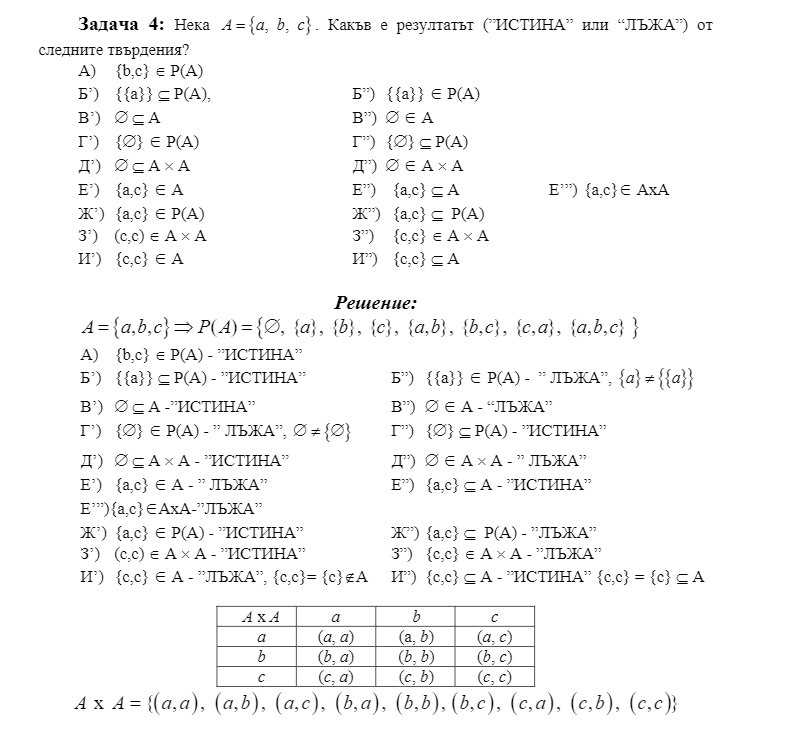
\includegraphics{Pics/Discrete math/ex3/ex3-task4.png}
\end{figure}
\newpage
\begin{figure}[h!]
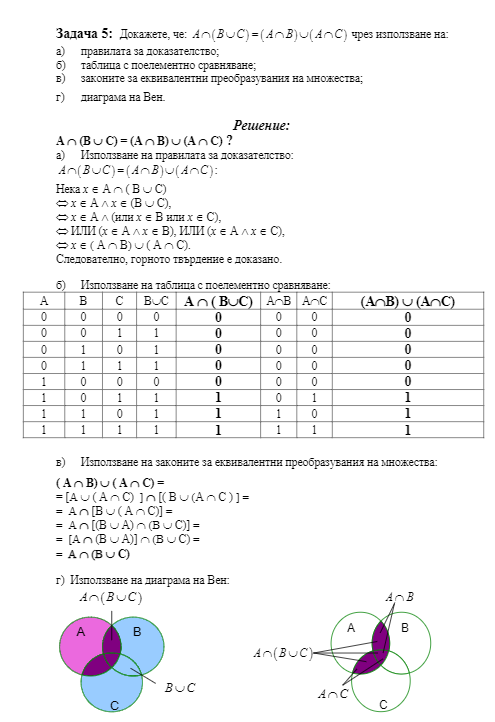
\includegraphics{Pics/Discrete math/ex3/ex3-task5.png}
\end{figure}

\newpage
\subsubsection*{Задача 9}
Истина или лъжа е следното твърдение $A \otimes (B \otimes C) = (A \otimes B) \otimes C$
\begin{table}[htp]
\begin{center}
\begin{tabular}{|c|c|c|c|c|c|c|} 
\hline
 A & B & C  & $A \otimes B$ & $B \otimes C$ & $A \otimes (B \otimes C)$ & $(A \otimes B) \otimes C$  \\
\hline
0 & 0 & 0 & 0 & 0 & 0 & 0 \\
\hline
0 & 0 & 1 & 0 & 1 & 1 & 1 \\
\hline
0 & 1 & 0 & 1 & 1 & 1 & 1 \\
\hline
0 & 1 & 1 & 1 & 0 & 0 & 0 \\
\hline
1 & 0 & 0 & 1 & 0 & 1 & 1 \\
\hline
1 & 0 & 1 & 1 & 1 & 0 & 0 \\
\hline
1 & 1 & 0 & 0 & 1 & 0 & 0 \\
\hline
1 & 1 & 1 & 0 & 0 & 1 & 1 \\
\hline
\end{tabular}
\end{center}
\end{table}
\newpage

\subsubsection*{Задача 10}
Какъв ще е резултатът от следните твърдения?
\begin{enumerate}
\item $A - (B - C) = (A - B) - C$
\item $(A-C) - (B-C) = A - B$
\item $A \cup (B \cap C) = (A \cup B) \cap (A \cup C)$
\item $A \cap (B \cup C) = (A \cap B) \cup (A \cap C)$
\item $A\cup C = B \cup C \implies A = B$
\item $A\cap C = B \cap C \implies A = B$
\item $A \otimes B = A \implies B =A$
\end{enumerate}

\begin{figure}[h!]
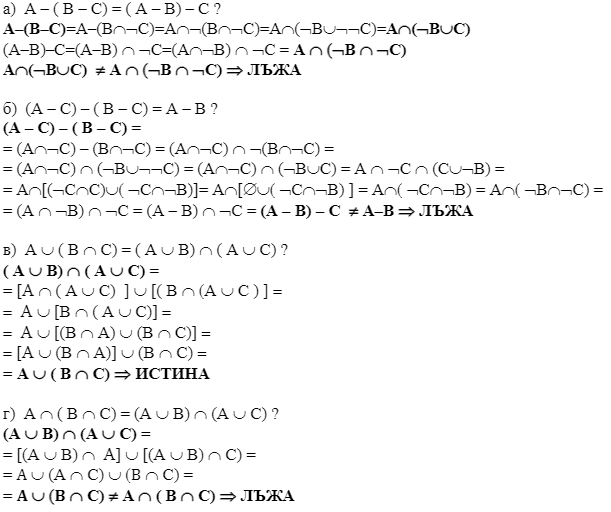
\includegraphics{Pics/Discrete math/ex3/ex3-task10-1.png}
\end{figure}

\begin{figure} 
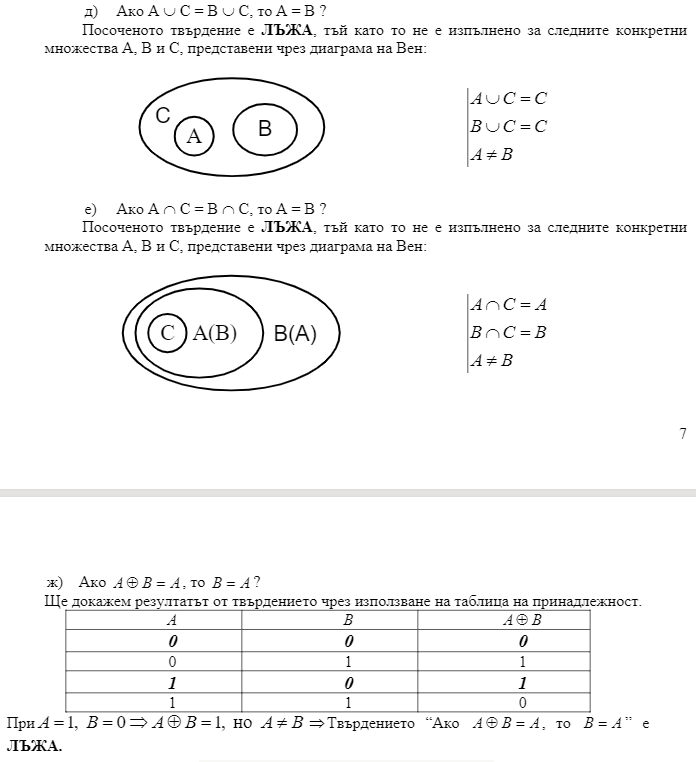
\includegraphics{Pics/Discrete math/ex3/ex3-task10-2.png}
\end{figure}

\newpage
\subsection{Упражнение 4: Математически доказателства}

\subsubsection*{Задача 1}
За  всеки  от  следващите  аргументи  кои  правила  за  доказателство  са използвани на всяка стъпка?
\begin{enumerate}
\item "Студентката от ТУ-София Петя има собствена кола. Всеки, който има кола, пътува по-удобно и по-бързо. Следователно, съществува студент от ТУ-София, който пътува по-удобно и по-бързо."
\item "Всеки от петимата студенти от ТУ-София Иван, Георги, Петър, Стоян и Никола е взел успешно изпита по ТЕ-1.  Всеки студент, който е взел успешно ТЕ-1 има право да се яви на изпит по ТЕ-2. Следователно, и петте гореспоменати момчета могат да се явят на изпит по ТЕ-2 през лятната сесия."
\end{enumerate}
Решение:
\begin{enumerate}
\item Нека: X - множество на всички студенти, x- произволен студент\\
c(x) - "х е студент от ТУ-София."\\
p(x) - "х    има собствена кола"\\
s(x) - "x се придвижва по-удобно и по-бързо."\\
Доказателство: \\
Изходни хипотези: c(Петя), p(Петя) и$\forall x( p(x) \to s(x) )$. \\
Заключение:$\exists x( c(x) \land s (x) )$.
\begin{enumerate}
\item $\forall x( p(x) \to s(x) ) \quad$ Хипотеза
\item p(Петя) $\to$ s(Петя) $\quad$ Универсално следствие (Universal instantiation) от а
\item p(Петя) $\quad$ Хипотеза
\item s(Петя) $\quad$ Закон на безразличие (Modus Ponens) от б и в 
\item c(Петя) $\quad$ Хипотеза
\item c(Петя) $\land$ s(Петя)  $\quad $ Конюнкция ( Conjunction)от г и д 
\item $\exists x( c(x) \land s (x) ) \quad$ Частично обобщение (Existential generalisation) от е
\end{enumerate}
\item Нека: X  – множест  во от всички студенти в ТУ-София; x  – произволен студентот X.\\ 
f(x) - "x е един от петимата студенти Иван, Георги, Петър, Стоян и Никола."\\
$t_1(x)$ - "x е взел успешно изпита по ТЕ-1."\\
$t_2(x)$ - "x има право да се яви на изпит по ТЕ-2."\\
y - произволен студент от петиматапо-горе. \\
Изходни хипотези:$\forall x(f(x) \to t_1(x))$ и$\forall x(t_1(x) \to  t_2(x))$ \\
Заключение:$\forall x(f(x) \to t_2(x))$. \\
Доказателство:
\begin{enumerate}
\item $\forall x(f(x) \to t_1(x)) \quad $ Хипотеза 
\item $f(y) \to t_1(x) \quad $ Универсално следствие (Universal instantiation) от а
\item $\forall x(t_1(x) \to  t_2(x)) \quad  $ Хипотеза
\item $t_1(y) \to  t_2(y) \quad $ Универсално следствие (Universal instantiation) от в
\item $f(y) \to  t_2(y) \quad $ Хипотетичен силогизъм (Hypothetical syllogism) от б и г
\item $\forall x(f(x) \to t_2(x)) \quad $ Универсално обобщение (Universal generalisation) от д 
\end{enumerate}
\end{enumerate}

\subsubsection*{Задача 2}
Коректно ли е доказателството на следния аргумент: "Ако $n^2$ не се дели на 3, то n също не е кратно на 3?"\\ Доказателство: " Ако $n^2$ не се дели на 3, тогава $n^2 \neq 3k, k =0, 1, ...$. Следователно $n \neq 3l, l=0, 1, ...$, откъдето следва, че n не е кратно на 3."\\
Решение \\
От  горното  доказателство  се  вижда,  че  от  това,  че $n^2 \neq 3k, k =0, 1, ...$ не  следва директно, че $n \neq 3l, l=0, 1, ...$ а трябва да се докаже. \\
За целта ще използваме индиректно доказателство: “Ако n е кратно на 3, то $n^2$ също се дели на 3.” \\
Ако допуснем, че n е кратно на 3 $\implies$ 
$$n = 3l \implies n^2 = (3l)^2 = 3(3l)^2 = 3k \implies n^2$$
Откъдето следва, че горепосоченият аргумент е верен, но посоченото доказателство е некоректно.

\subsubsection*{Задача 3}
Да се докаже, че квадратът на всяко четно число е също четно число чрез:
\begin{enumerate}
\item директно доказателство
\item индиректно доказателство
\item използване на контра-пример
\end{enumerate}
Хипотеза p : "n е четно число."
Заключение q: "$n^2$ е четно число."
\begin{enumerate}
\item директно доказателство $p \to q$\\
Нека n е  четно  число $\implies$ то  може  да  се  запише  като:
$$n = 2k, k =0, 1, ... \implies n^2 = (2k)^2 = 4k^2 = 2(2k^2) \implies n^2$$ 

\item индиректно доказателство $(\neg p \to \neg q) \Leftrightarrow (p \to q)$\\
Нека $n^2$ е нечетно число $\implies$ то може да се запише като: 
$$n^2 = 2k+1, k =0, 1, ... $$
$\implies$  n е нечетно число.

\item използване на контра-пример \\
"Ако $n^2$ е нечетно число, то nсъщо е нечетно число." \\
Хипотеза 1: "$n^2$ е нечетно число." - p \\
Хипотеза 2:  "n е четно число." -  $\overline{q} $\\
Допускаме, че Хипотеза 2 $\overline{q} $ е вярна $\implies$
$$n =2k, k =0, 1, ... \implies n^2 = (2k)^2 = 2(2k^2) \implies n^2 = 2l \implies n^2$$
 e четно число, т.е. $\overline{p} $, което е в противоречие с Хипотеза 1 p $\implies$
Допускането е грешно $\implies$ Хипотеза 2 не е вярна $\implies$ "n е нечетно число."
\end{enumerate}

\subsubsection*{Задача 4}
Да се докаже, че произведението на две рационални числa е също рационално числo.\\
Решение \\
Директно доказателство: Нека а и b са рационални числа $\implies$ те могат да се запишат във вида 
$$a = \frac{k}{l} \quad b = \frac{s}{t} \qquad k,l,s,t \in \mathbb{Z}, l \neq 0, s \neq 0 \implies ab = \frac{ks}{lt}$$

\subsubsection*{Задача 5}
Вярно е, че произведението на две ирационални числа е ирационално число?\\
Решение\\
Aко $a = b = \sqrt{2} \implies ab = 2$ което е рационално число $\implies$ твърдението е лъжа.

\subsubsection*{Задача 6}
Да се докаже, че следващите три твърдения са еквивалентни при $n \in Z$.
\begin{enumerate}
\item n е четно число.
\item n+1 е нечетно число.
\item 3n+1 е нечетно число.
\end{enumerate}
$1 \to 2$\\
$$n = 2k \implies n+1 = 2k + 1 , k \in \mathbb{N}$$
$2 \to 3$\\
$$n+1 = 2k + 1 \implies 3n + 1 = 3(2k) + 1 = 2(3k) + 1 = 3n + 1, k \in \mathbb{N}$$
$3 \to 1$\\
$$3n + 1 = 2k + 1 \implies 3n = 2k, 2k = 2t \implies n = 2k , k,t \in \mathbb{N}$$

\subsubsection*{Задача 7}
Да се докаже, че $\sqrt[3]{3}$ е ирационално число! \\
Решение\\
$a \in \mathbb{Z}, b \in \mathbb{Z}$ a,b - взаимно прости(Най голям общ делител = 1)\\
$$\frac{a}{b} = \sqrt[3]{3} \implies \left( \frac{a}{b}\right)^3 = 3 \implies a^3 = 3b^3$$
$a^3$ е кратно на 3 $\implies$ a се дели на 3 $\implies$
$$a = 3k, k \in \mathbb{N} \implies 3b^3 = a^3 = (3k)^3 = 9k^3 \implies b^3 = 9k^3 = 3s, s \in \mathbb{N}$$
$b^3$ е кратно на 3 $\implies$ b се дели на 3 $\implies$
$$b = 3l, l \in \mathbb{N} \implies \frac{a}{b} = \frac{3k}{3l} \implies$$
a и b не са взаимно прости числа (най-големият им общ делител е 3), както допуснахме по-горе $\implies$ Хипотезата, e лъжа $\implies$ $\sqrt[3]{3}$ е ирационално число

\newpage
\subsection{Упражнение 5: Булева алгебра}

\subsubsection*{Задача 1}
Нека функцията $f(x,y,z)$ е дефинирана посредством следната таблица:
\begin{table}[htp]
\begin{center}
\begin{tabular}{|c|c|c|c|c|} 
\hline
  &  &   & а  & б \\
\hline
x & y & z & f(x,y,z) & f(x,y,z) \\
\hline
0 & 0 & 0 & 1 & 0 \\
\hline
0 & 0 & 1 & 0 & 1 \\
\hline
0 & 1 & 0 & 1 & 0 \\
\hline
0 & 1 & 1 & 0 & 0 \\
\hline
1 & 0 & 0 & 0 & 1 \\
\hline
1 & 0 & 1 & 0 & 1 \\
\hline
1 & 1 & 0 & 1 & 0 \\
\hline
1 & 1 & 1 & 1 & 1 \\
\hline
\end{tabular}
\end{center}
\end{table}
Да се намери съответни аналитични изрази!  \\
a) $f(x,y,z) = (-x) \cdot (-y) \cdot (-z) +(-x) \cdot y \cdot (-z) + x \cdot y \cdot (-z) + x \cdot y \cdot z$  \\
б) $f(x,y,z) = (-x) \cdot (-y) \cdot z + x \cdot (-y) \cdot(-z) + x \cdot (-y) \cdot z + x \cdot y \cdot z$
\subsubsection*{Задача 2}
Истина или лъжа са следните твърдения 
\begin{enumerate}
\item $(a \vert b = b \vert a) \Leftrightarrow a = b$ 
\begin{table}[htp]
\begin{center}
\begin{tabular}{|c|c|c|c|} 
\hline
a & b & $a \vert b$ & $b \vert a$\\
\hline
0 & 0 & 1 & 1 \\
\hline
0 & 1 & 1 & 1 \\
\hline
1 & 0 & 1 & 1 \\
\hline
1 & 1 & 0 & 0 \\
\hline
\end{tabular}
\end{center}
\end{table}
\item $(a \vert b) \cdot (c \vert d) \Leftrightarrow (a+c) \vert (b+d) $
\begin{equation}
(a \vert b) \cdot (c \vert d) =
 (\overline{a \cdot b}) \cdot (\overline{c \cdot d}) = 
(\overline{a} + \overline{b}) \cdot (\overline{c} + \overline{d}) = 
\overline{a} \cdot \overline{c} + \overline{a} \cdot \overline{d} + \overline{b} \cdot \overline{c} + \overline{b} \cdot \overline{d}
\end{equation}
\begin{equation}
(a+c) \vert (b+d) = 
\overline{(a+c) \cdot (b+d)} =
\overline{a+c} + \overline{b + d} = 
\overline{a} \cdot \overline{c} + \overline{b} \cdot \overline{d}
\end{equation}
От (1) и (2) $\implies (a \vert b) \cdot (c \vert d) \neq (a+c) \vert (b+d)$
\end{enumerate}
\newpage
\subsection{Упражнение 6: Релации }

\subsubsection*{Задача 1}
Да се провери дали всяка от бинарните релации е\\
рефлексивна/антирефлексивна/симетрична/асиметрична/антисиметрична/транзитивна:
\begin{enumerate}
\item Релация R върху множествотo N, където $(a,b) \in R $ тогава и само тогава когато $a \land b$
\begin{figure} [htp!]
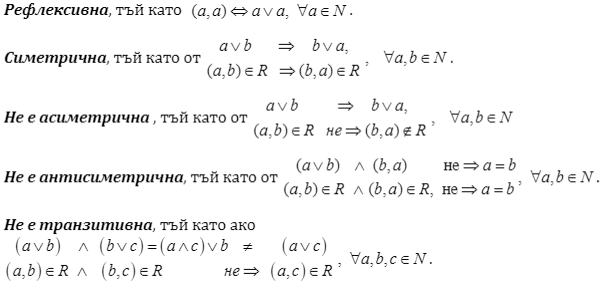
\includegraphics[width=\linewidth]{Pics/Discrete math/ex6/ex6-task1-1.png}
\end{figure}
\item Релация R върху множеството S = \{w,x,y,z \}, където 
$$R = \{ (w, w), (w, x), (x, w), (x, x), (x, z), (y, y), (z, y), (z, z) \}$$
\begin{figure} [htp!]
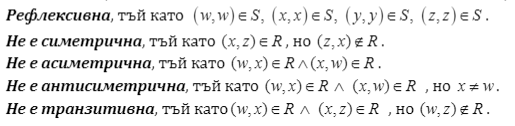
\includegraphics[width=\linewidth]{Pics/Discrete math/ex6/ex6-task1-2.png}
\end{figure}
\item Релация R върху множеството $P(x)$ на  множеството X = \{ 1, 2, 3, 4\} където $(S,T) \in R$ тогава и само тогава когато $S \subseteq T$
\begin{figure} [htp!]
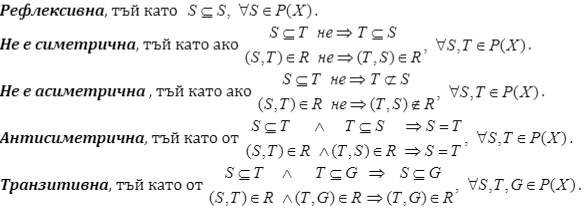
\includegraphics[width=\linewidth]{Pics/Discrete math/ex6/ex6-task1-3.png}
\end{figure}
\end{enumerate}

\subsubsection*{Задача 2}
Нека R и S са релации oт вида
$$R = \{(1, 2), (1, 3), (2, 3), (2, 4), (3, 4) \} \qquad S = \{(2, 1), (3, 1), (3, 2), (4, 2)\}$$
Да се определи композицията им $S \circ R$ \\
Решение \\
$$(b,c) \circ (a,b) = (a,c) $$
$$S \circ R = \{ (1, 1), (2, 1), (2, 1), (2, 2) \}$$

\newpage
\subsubsection*{Задача 3}
\begin{figure} [htp!]
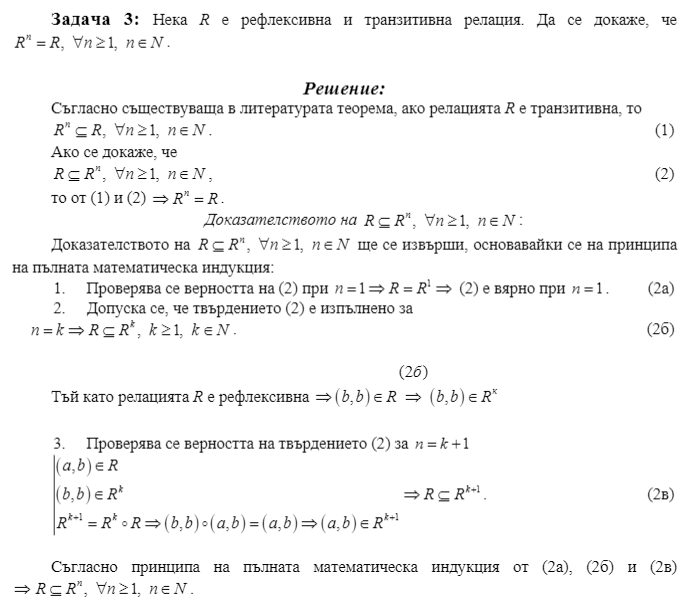
\includegraphics[width=\linewidth]{Pics/Discrete math/ex6/ex6-task3.png}
\end{figure}

\newpage
\subsubsection*{Задача 4}
Да се състави матрица, описваща следната релация R върху множеството \{1,2,3,4\}, където $(a,b) \in R $, тогава и само тогава когато $\vert a - b \vert \leq 1$ \\
Решение : \\
\begin{figure} [htp!]
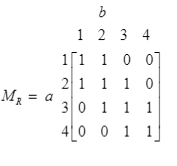
\includegraphics{Pics/Discrete math/ex6/ex6-task4.png}
\end{figure}

\subsubsection*{Задача 5}
Ако релациите R и S се представят със следните матрици
$$M_R = 
\begin{bmatrix}
1 & 0 & 0\\
1 & 1 & 0 \\
1 & 1 & 0 
\end{bmatrix} 
\quad
M_S = 
\begin{bmatrix}
0 & 0 & 1\\
0 & 1 & 0 \\
1 & 1 & 0 
\end{bmatrix}  
$$
Определете матриците, които представят $R \cup S$ и $R \cap S$? \\
Решение: \\
$$
M_{R \cup S} = M_R \lor M_S = 
\begin{bmatrix}
1 & 0 & 1\\
1 & 1 & 0\\
1 & 1 & 0
\end{bmatrix}
\qquad
M_{R \cap S} = M_R \land M_S =
\begin{bmatrix}
0 & 0 & 0\\
0 & 1 & 0\\
1 & 1 & 0
\end{bmatrix}
$$
\newpage
\subsubsection*{Задача 6}
Да се определи релацията по следната матрица
\begin{figure} [htp!]
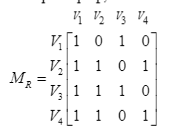
\includegraphics{Pics/Discrete math/ex6/ex6-task6.png}
\end{figure}
$$R = \{(1, 1), (1, 3), (2, 1), (2, 2), (2, 4), (3, 1), (3, 2), (3, 3), (4, 1), (4, 2), (4, 4) \}$$
\subsubsection*{Задача 7}
\begin{figure} [htp!]
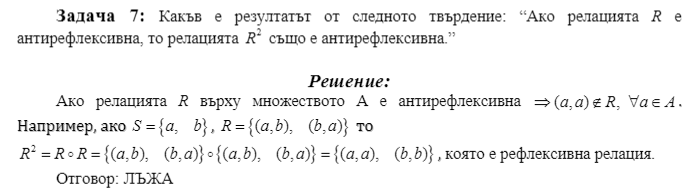
\includegraphics[width=\linewidth]{Pics/Discrete math/ex6/ex6-task7.png}
\end{figure}

\newpage
\subsection{Упражнение 7: Функции и суми}

\subsubsection*{Задача 1}
Нека са дадени следните множества \\
$
A = \{1, 2, 3, 4\} \\
B = \{ a, b, c\} \\
C = \{2, 7, 10 \}
$
На тяхна основа са дефинирани функциите \\
$$g: A \to B \qquad f: B \to C$$
по следния начин
$$g = \{ (1, b), (2, a), (3, c) \} \qquad f = \{ (a, 10), (b, 7), (c, 2) \}$$
Композицията $f \circ g$ е \\
$$ f \circ g = \{ (1, b), (2, a), (3, c) \} \circ  \{ (a, 10), (b, 7), (c, 2) \} = \{ (1, 7), (2, 10), (3, 2) \}$$

\subsubsection*{Задача 2}
Да се намерят обратните функции $f^{-1}$ на следните функции f:
\begin{enumerate}
\item $f: A \to B, \, A = \{ a, b, c \}, \, B = \{2, 7, 10 \}, \, f = \{ (a, 10), (b, 7), (c, 2) \}$
$\forall x \in A \implies \exists y \in B, f(x) = y$\\
f е инекция, f e сюрекция $\implies$ f е биекция $\implies$
$$f^{-1} = \{ (10, a), (7, b), (2, c) \}$$
\item $f: A \to B$, A = \{ Иван, Стоян, Георги, Тони \}, \\
B = \{ Опел, Форд, Рено, Пежо, Ситроен \},\\ 
f= \{ (Иван, Пежо), (Стоян, Форд), (Георги, Рено), (Тони, Опел) \} \\
$\forall a \in A \implies \exists b \in B, f(a) = b$ \\
$f(\varnothing) = \text{Ситроен}$\\
f е инекция, f не e сюрекция $\implies $ f не е биекция$\implies \centernot\exists f^{-1}$ 
\item $f: \mathbb{R} \to \mathbb{R}, \, f(x) = 3x + 5$ \\
f е инекция, f e сюрекция $\implies$ f е биекция $\implies \exists f^{-1}$
$$x = 3y + 5 \implies y = f^{-1}(x) = \frac{x-5}{3} $$
\item $f: \mathbb{R} \to \mathbb{R}, \, x > \frac{2}{7}, \, f(x) = \ln{(7x-2)}$\\
f е инекция, f e сюрекция $\implies$ f е биекция $\implies \exists f^{-1}$
$$x = \ln{(7y-2)} \implies 7y - 2 = e^x \implies y = f^{-1}(x) = \frac{e^x + 2}{7}$$
\end{enumerate}

\subsubsection*{Задача 3}
Да се запишат нулевия, първия, втория и третия член на редица с общ член $a_n$ от вида:
\begin{enumerate}
\item $(-2)^n$\\
$$a_0 = (-2)^0 = 1, \  a_1 = (-2)^1 = -2, \  a_2 = (-2)^2 = 4, \ a_3 = (-2)^3 = -8$$
\item 3\\
$$a_0 = a_1 = a_2 = a_3 = 3$$
\item $7 + 4^n$\\
$$a_0 = 7 + 4^0 = 8, \ a_1 = 7 + 4^1 = 11, \ a_2 = 7 + 4^2 = 23,  \ a_3 = 7 + 4^3 = 71 $$
\item $2^n + (-2)^n$\\
$$a_0 = 2^0 + (-2)^0 = 2 \qquad a_1 = 2^1 + (-2)^1 = 0$$
$$ a_2 = 2^2 + (-2)^2 = 8 \qquad  a_3 = 2^3 + (-2)^3 = 0$$
\end{enumerate}

\subsubsection*{Задача 4}
Да се запише общият член $a_n$ за всеки от посочените редове от цели числа $(n \geq 1, n \in \mathbb{N})$
\begin{enumerate}
\item $ 7, 11, 15, 19, 23, 27, 31, 35, 39, 43, ... $ - аритметична прогресия
$$a_1 = 7 \qquad d = 4 \implies a_n = a_1 +(n-1)d = 7 + (n-1)4$$
\item $ 2, 6, 18, 54, 162, 486, 1458, 4374, 13122, 39366, ... $ - геометрична прогресия
$$a_1 = 2 \qquad q = 3 \implies a_n = a_1 \cdot q^{n-1} = 2 \cdot 3^{n-1}$$
\item $ 3, 6, 11, 18, 27, 38, 51, 66, 83, 102, ... $
$$a_1 = 3 \quad a_2 = 6 = a_1 + 3 \quad a_3 = 11 = a_2 + 5 \quad a_4 = 18 = a_3 + 7$$
$$a_{n-1} = a_{n-2} + (2(n-1) - 1) = a_{n-2} + (2n - 3)$$
$$a_n = a_{n-1} + (2n-1)$$
$$a_n = 3+(3+5+...+(2n-1)) = 2 + (1+3+5+...+(2n-1)) = $$
$$2 + \frac{(1+2n-1)n}{2} = 2 + \frac{2n \cdot n}{2} = n^2 + 2$$
\end{enumerate}

\subsubsection*{Задача 5}
Да се намери стойността на всяка от следните суми:
\begin{enumerate}
\item $S_9 = \sum_{k=0}^8 (1 + (-1)^k)$
$$S_9 = \sum_{k=0}^8 (1 + (-1)^k) = 2 + 0 + 2 + 0 + 2 + 0 + 2 + 0 + 2 = 5 \cdot 2 + 4 \cdot 0 = 10$$
\item $S_4 = \sum_{k=0}^4 (2^k + 3k)$
$$S_4 = \sum_{k=0}^4 (2^k + 3k) = \sum_{k=0}^4 2^k + \sum_{k=0}^4 3k = \sum_{k=0}^4 2^k + 3\sum_{k=0}^4 k$$
$$a_{1geo} \cdot \frac{q^4 - 1}{q -1} + 3 \frac{4(a_{1alg} + a_{4alg})}{2} = 2 \cdot \frac{2^4 - 1}{2 -1} + 3 \frac{4(1 +4)}{2} =  \frac{2 \cdot 15}{1} + \frac{3 \cdot 4 \cdot 5}{2} = 30 + 30 = 60$$
\item $S_5 = \sum_{k=0}^4 5 \cdot 2^k$
$$S_5 = \sum_{k=0}^4 5 \cdot 2^k = 5 \sum_{k=0}^4 2^k = 5 \cdot a_0  \frac{q^5 - 1}{q -1} = 5 \cdot 2^0 \frac{2^5 - 1}{2 -1} = 5 \cdot 31 = 155$$
\item $S = \sum_{i=0}^2 \sum_{j=0}^3 (2i + 3j)$
$$S = \sum_{i=0}^2 \sum_{j=0}^3 (2i + 3j) = \sum_{i=0}^2 \sum_{j=0}^3 2i + \sum_{i=0}^2 \sum_{j=0}^3 3j = $$ $$4 \cdot 2 \sum_{i=0}^2 i + 3 \cdot 3 \sum_{j=0}^3 j = 8 \cdot \frac{(0+2)3}{2} + 9 \cdot \frac{(0+3)4}{2} = 24 + 54 = 78$$
\end{enumerate}

\newpage
\subsubsection*{Задача 6}
\begin{figure} [htp!]
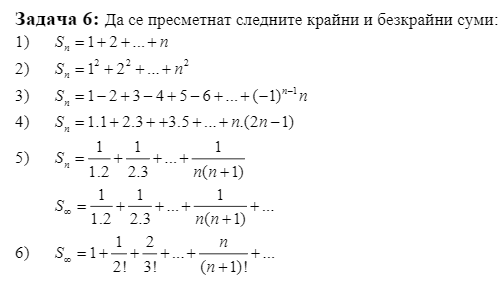
\includegraphics[width = \linewidth]{Pics/Discrete math/ex7/ex7-task6-1.png}
\end{figure}
\begin{figure} [htp!]
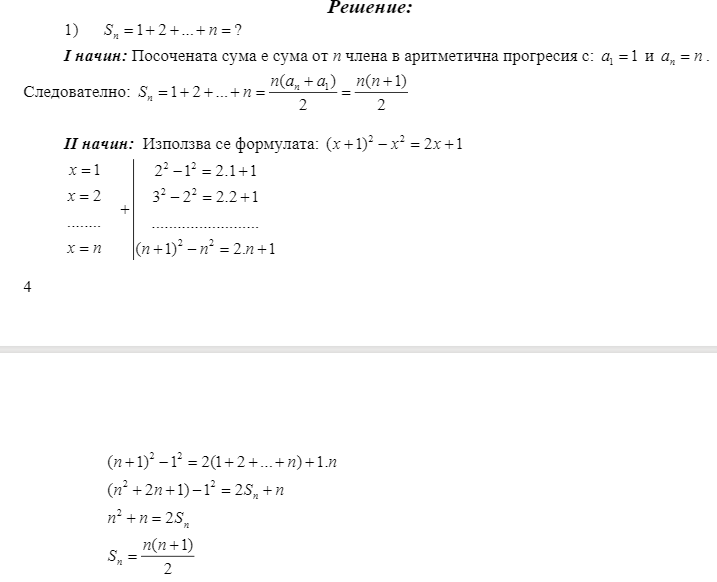
\includegraphics{Pics/Discrete math/ex7/ex7-task6-2.png}
\end{figure}
\begin{figure} [htp!]
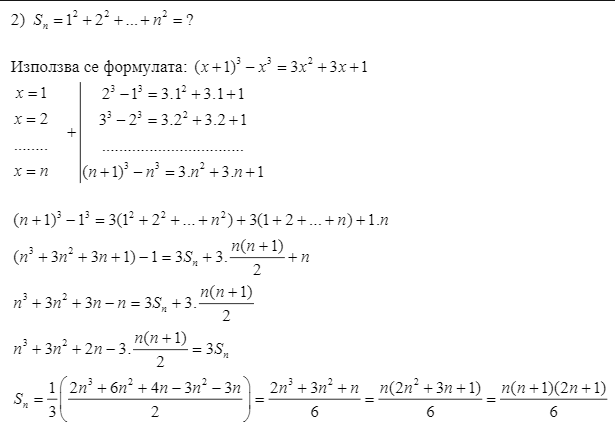
\includegraphics{Pics/Discrete math/ex7/ex7-task6-3.png}
\end{figure}
\begin{figure} [htp!]
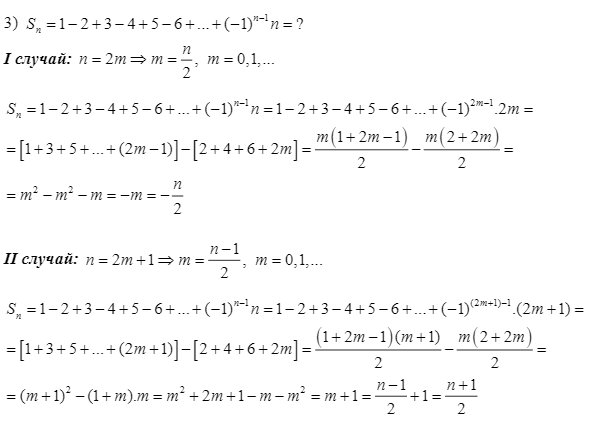
\includegraphics{Pics/Discrete math/ex7/ex7-task6-4.png}
\end{figure}
\begin{figure} [htp!]
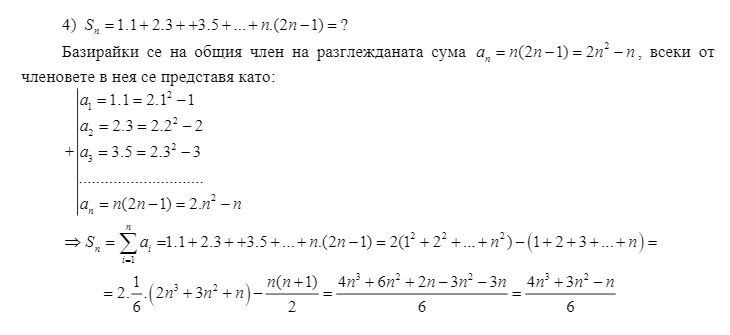
\includegraphics{Pics/Discrete math/ex7/ex7-task6-5.png}
\end{figure}
\begin{figure} [htp!]
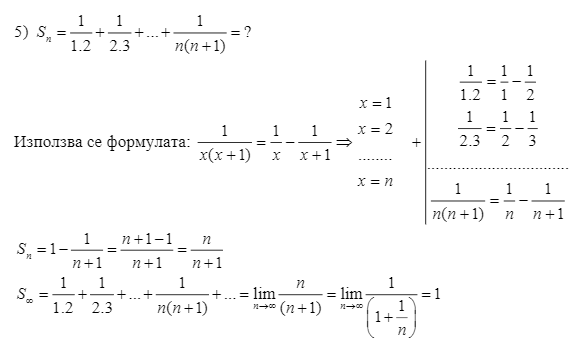
\includegraphics{Pics/Discrete math/ex7/ex7-task6-6.png}
\end{figure}
\begin{figure} [htp!]
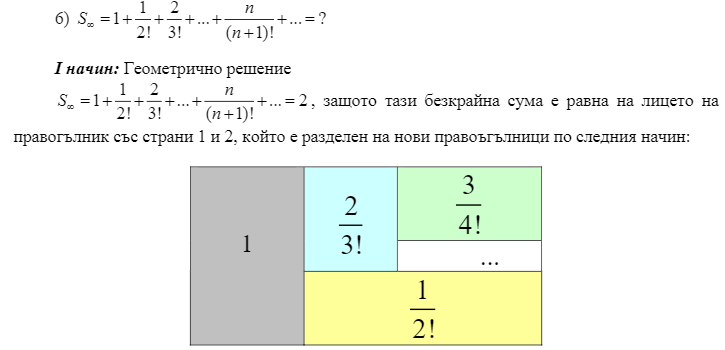
\includegraphics{Pics/Discrete math/ex7/ex7-task6-7.png}
\end{figure}
\begin{figure} [htp!]
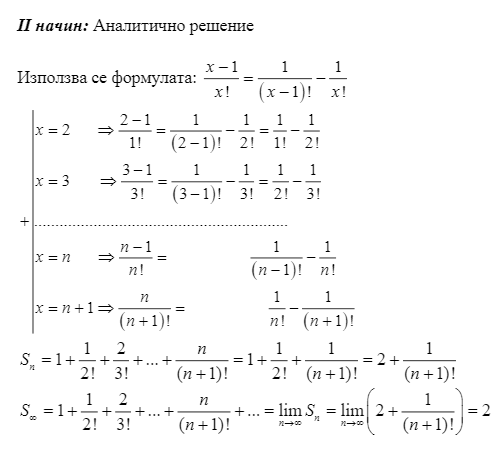
\includegraphics{Pics/Discrete math/ex7/ex7-task6-8.png}
\end{figure}

\newpage
\subsection{Упражнение 8: Графи и дървета}

\subsubsection*{Задача 1}
\begin{figure} [htp!]
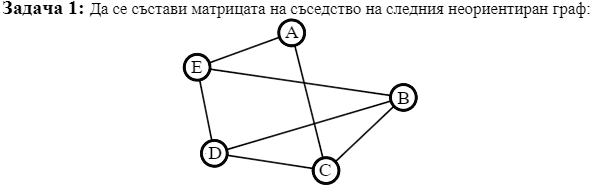
\includegraphics[width = \linewidth]{Pics/Discrete math/ex8/ex8-task1.png}
\end{figure}
$$A_G = 
\begin{bmatrix}
0 & 0 & 1 & 1 & 0 \\
0 & 0 & 1 & 1 & 1 \\
1 & 1 & 0 & 1 & 0 \\
0 & 1 & 1 & 0 & 1 \\
1 & 1 & 0 & 1 & 0 \\
\end{bmatrix}
$$
Извод: Матрицата на съседство на неориентиран граф е симетрична квадратна матрица, чиито елементи $(i,i)$по главния диагонал са 1, ако около съответния връх $V_i$ има примка.
\subsubsection*{Задача 2}
\begin{figure} [htp!]
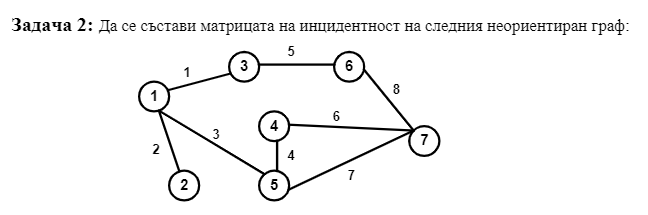
\includegraphics[width = \linewidth]{Pics/Discrete math/ex8/ex8-task2.png}
\end{figure}
$$A_I = 
\begin{bmatrix}
1 & 1 & 1 & 0 & 0 & 0 & 0 & 0 \\
0 & 1 & 0 & 0 & 0 & 0 & 0 & 0 \\
1 & 0 & 0 & 0 & 1 & 0 & 0 & 0 \\
0 & 0 & 0 & 1 & 0 & 1 & 0 & 0 \\
0 & 0 & 1 & 1 & 0 & 0 & 1 & 0 \\
0 & 0 & 0 & 0 & 1 & 0 & 0 & 1 \\
0 & 0 & 0 & 0 & 0 & 1 & 1 & 1 \\
\end{bmatrix}
$$
Извод: Матрицата на инцидентност на неориентиран граф съдържа по две 1 в колона, съответстваща на нормално ребро и по една 1 в колона, съответстваща на ребро-примка.
\subsubsection*{Задача 3}
\begin{figure} [htp!]
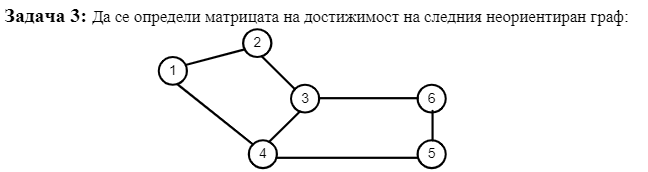
\includegraphics[width = \linewidth]{Pics/Discrete math/ex8/ex8-task3.png}
\end{figure}

\begin{gather*}
I = 
\begin{bmatrix}
1 & 0 & 0 & 0 & 0 & 0 \\
0 & 1 & 0 & 0 & 0 & 0 \\
0 & 0 & 1 & 0 & 0 & 0 \\
0 & 0 & 0 & 1 & 0 & 0 \\
0 & 0 & 0 & 0 & 1 & 0 \\
0 & 0 & 0 & 0 & 0 & 1  \\
\end{bmatrix} 
\quad 
A_G = 
\begin{bmatrix}
0 & 1 & 0 & 1 & 0 & 0 \\
1 & 0 & 1 & 0 & 0 & 0 \\
0 & 1 & 0 & 1 & 0 & 1 \\
1 & 0 & 1 & 0 & 1 & 0 \\
0 & 0 & 0 & 1 & 0 & 1 \\
0 & 0 & 1 & 0 & 1 & 0  \\
\end{bmatrix} 
\quad
H_1 = I \cup A_G = 
\begin{bmatrix}
1 & 1 & 0 & 1 & 0 & 0 \\
1 & 1 & 1 & 0 & 0 & 0 \\
0 & 1 & 1 & 1 & 0 & 1 \\
1 & 0 & 1 & 1 & 1 & 0 \\
0 & 0 & 0 & 1 & 1 & 1 \\
0 & 0 & 1 & 0 & 1 & 1  \\
\end{bmatrix} \\
A_G^2 = A_G \cdot A_G = 
\begin{bmatrix}
0 & 1 & 0 & 1 & 0 & 0 \\
1 & 0 & 1 & 0 & 0 & 0 \\
0 & 1 & 0 & 1 & 0 & 1 \\
1 & 0 & 1 & 0 & 1 & 0 \\
0 & 0 & 0 & 1 & 0 & 1 \\
0 & 0 & 1 & 0 & 1 & 0  \\
\end{bmatrix}
\cdot
\begin{bmatrix}
0 & 1 & 0 & 1 & 0 & 0 \\
1 & 0 & 1 & 0 & 0 & 0 \\
0 & 1 & 0 & 1 & 0 & 1 \\
1 & 0 & 1 & 0 & 1 & 0 \\
0 & 0 & 0 & 1 & 0 & 1 \\
0 & 0 & 1 & 0 & 1 & 0  \\
\end{bmatrix}
= 
\begin{bmatrix}
1 & 0 & 1 & 0 & 1 & 0 \\
0 & 1 & 0 & 1 & 0 & 1 \\
1 & 0 & 1 & 0 & 1 & 0 \\
0 & 1 & 0 & 1 & 0 & 1 \\
1 & 0 & 1 & 0 & 1 & 0 \\
0 & 1 & 0 & 1 & 0 & 1  \\
\end{bmatrix} 
\end{gather*}
\begin{gather*}
A_G^3 = A_G^2 \cdot A_G = 
\begin{bmatrix}
1 & 0 & 1 & 0 & 1 & 0 \\
0 & 1 & 0 & 1 & 0 & 1 \\
1 & 0 & 1 & 0 & 1 & 0 \\
0 & 1 & 0 & 1 & 0 & 1 \\
1 & 0 & 1 & 0 & 1 & 0 \\
0 & 1 & 0 & 1 & 0 & 1  \\
\end{bmatrix} 
\cdot 
\begin{bmatrix}
0 & 1 & 0 & 1 & 0 & 0 \\
1 & 0 & 1 & 0 & 0 & 0 \\
0 & 1 & 0 & 1 & 0 & 1 \\
1 & 0 & 1 & 0 & 1 & 0 \\
0 & 0 & 0 & 1 & 0 & 1 \\
0 & 0 & 1 & 0 & 1 & 0  \\
\end{bmatrix}
= 
\begin{bmatrix}
0 & 1 & 0 & 1 & 0 & 1 \\
1 & 0 & 1 & 0 & 1 & 0 \\
0 & 1 & 0 & 1 & 0 & 1 \\
1 & 0 & 1 & 0 & 1 & 0 \\
0 & 1 & 0 & 1 & 0 & 1 \\
1 & 0 & 1 & 0 & 1 & 0  \\
\end{bmatrix}\\
H_2 = I \cup A_G \cup A_G^2 = H_1 \cup A_G^2 = 
\begin{bmatrix}
1 & 1 & 1 & 1 & 1 & 0 \\
1 & 1 & 1 & 1 & 0 & 1 \\
1 & 1 & 1 & 1 & 1 & 1 \\
1 & 1 & 1 & 1 & 1 & 1 \\
1 & 0 & 1 & 1 & 1 & 1 \\
0 & 1 & 1 & 1 & 1 & 1  \\
\end{bmatrix}\\
H_3 = I \cup A_G \cup A_G^2 \cup A_G^3 = H_2 \cup A_G^3 = 
\begin{bmatrix}
1 & 1 & 1 & 1 & 1 & 1 \\
1 & 1 & 1 & 1 & 1 & 1 \\
1 & 1 & 1 & 1 & 1 & 1 \\
1 & 1 & 1 & 1 & 1 & 1 \\
1 & 1 & 1 & 1 & 1 & 1 \\
1 & 1 & 1 & 1 & 1 & 1  \\
\end{bmatrix}
\end{gather*}
Елементите  на  матрицата $H_3$ са  само  от  1$\implies H_4 = H_3 \implies$ Процедурата  се  спира. \\
Всеки връх от разглеждания граф е достижим от всички останали.

\newpage
\subsubsection*{Задача 4}
\begin{figure} [htp!]
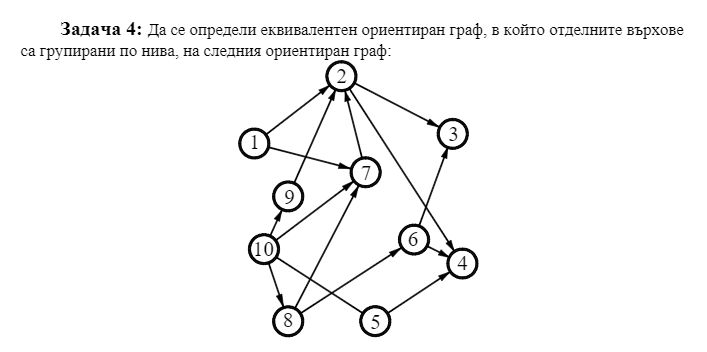
\includegraphics[width = \linewidth]{Pics/Discrete math/ex8/ex8-task4.png}
\end{figure}

\begin{enumerate}
\item За всеки връх $V_i$ се определя	множество $V^+ (i)$ от върхове, всеки от които е начало на дъга, влизаща във върха $V_i$ както следва:
\begin{itemize}
\item $V^+ (1)  = \varnothing $
\item $V^+ (2) = \{ V_1, V_9, V_7 \}$
\item $V^+ (3) = \{ V_2, V_6 \}$
\item $V^+ (4) = \{ V_2, V_5, V_6 \}$
\item $V^+ (5) = \{ V_{10} \}$
\item $V^+ (6) = \{ V_8 \}$
\item $V^+ (7) = \{ V_1, V_10, V_8 \}$
\item $V^+ (8) = \{ V_{10} \}$
\item $V^+ (9) = \{ V_{10} \}$
\item $V^+ (10) = \varnothing $
\end{itemize}
\item Определя се множеството от върхове от нулево ниво, което включва всички висящи (начални) върхове: 
$$V^0 = \{ V_1, V_10\}$$
\item Определя се множеството от върхове от първо ниво, което включва върхове, които са директно свързани чрез дъги единствено с върхове от нулево ниво:
$$V^1 = \{V_9, V_8, V_5 \} \quad V_i \in  V^1 \quad V^+(i) = V_0$$
\item Oпределя се множеството от върхове от второ ниво, което включва върхове, които са директно свързани чрез дъги единствено с върхове от нулево и първо ниво:
$$V^2 = \{V_7, V_6 \} \quad V_i \in  V^2 \quad V^+(i) = V_1$$
\item Определя се множеството от върхове от трето ниво, което включва върхове,които са директно свързани чрез дъги с върхове от нулево, първо и второ ниво:
$$V^3 = \{V_2 \} \quad V_i \in  V^3 \quad V^+(i) = V_2$$
\item Определя се множеството от върхове от четвърто ниво, което включва върхове, които са директно свързани чрез дъги с върхове от нулево, първо, второ и трето ниво:
$$V^4 = \{V_3, V_9 \} \quad V_i \in  V^4 \quad V^+(i) = V_3$$
\item Преномерират се върховете в новия граф (не е задължително).
\end{enumerate}

\begin{figure} [htp!]
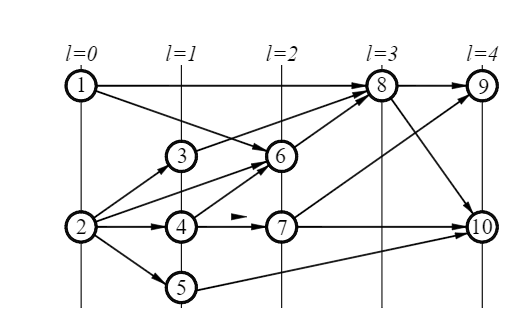
\includegraphics[width = \linewidth]{Pics/Discrete math/ex8/ex8-task4-1.png}
\end{figure}

\newpage
\subsubsection*{Задача 5}
\begin{figure} [htp!]
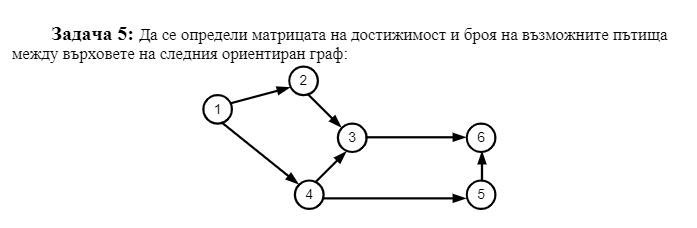
\includegraphics[width = \linewidth]{Pics/Discrete math/ex8/ex8-task5.png}
\end{figure}
\begin{enumerate}
\item Определя се еквивалентния ориентиран граф, в който отделните  върхове са групирани по нива, както следва:
\begin{figure} [htp!]
\centering
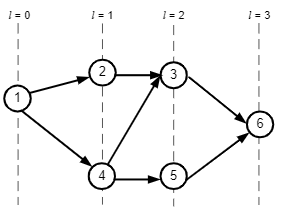
\includegraphics{Pics/Discrete math/ex8/ex8-task5-1.png}
\end{figure}
\item Формира се единична квадратна матрица от вида:
$$
I = 
\begin{bmatrix}
1 & 0 & 0 & 0 & 0 & 0 \\
0 & 1 & 0 & 0 & 0 & 0 \\
0 & 0 & 1 & 0 & 0 & 0 \\
0 & 0 & 0 & 1 & 0 & 0 \\
0 & 0 & 0 & 0 & 1 & 0 \\
0 & 0 & 0 & 0 & 0 & 1  \\
\end{bmatrix} 
\implies \quad 
H^0 = I = 
\begin{bmatrix}
1 & 0 & 0 & 0 & 0 & 0 \\
0 & 1 & 0 & 0 & 0 & 0 \\
0 & 0 & 1 & 0 & 0 & 0 \\
0 & 0 & 0 & 1 & 0 & 0 \\
0 & 0 & 0 & 0 & 1 & 0 \\
0 & 0 & 0 & 0 & 0 & 1  \\
\end{bmatrix} 
$$
\item Формира се матрицата на достижимост до върховете от ниво 1 -$H^1$: 
$$
H^{(0-1)} = 
\begin{bmatrix}
0 & 1 & 0 & 1 & 0 & 0 \\
0 & 0 & 0 & 0 & 0 & 0 \\
0 & 0 & 0 & 0 & 0 & 0 \\
0 & 0 & 0 & 0 & 0 & 0 \\
0 & 0 & 0 & 0 & 0 & 0 \\
0 & 0 & 0 & 0 & 0 & 0  \\
\end{bmatrix}
\implies \quad 
H^1 = H^{(0-1)} = 
\begin{bmatrix}
0 & 1 & 0 & 1 & 0 & 0 \\
0 & 0 & 0 & 0 & 0 & 0 \\
0 & 0 & 0 & 0 & 0 & 0 \\
0 & 0 & 0 & 0 & 0 & 0 \\
0 & 0 & 0 & 0 & 0 & 0 \\
0 & 0 & 0 & 0 & 0 & 0  \\
\end{bmatrix}
$$
\item Формира се матрицата на достижимост до върховете от ниво 2 -$H^2$:
$$
H^{(1-2)} = 
\begin{bmatrix}
0 & 0 & 0 & 0 & 0 & 0 \\
0 & 0 & 1 & 0 & 0 & 0 \\
0 & 0 & 0 & 0 & 0 & 0 \\
0 & 0 & 1 & 0 & 1 & 0 \\
0 & 0 & 0 & 0 & 0 & 0 \\
0 & 0 & 0 & 0 & 0 & 0  \\
\end{bmatrix}
\implies \quad 
H^2 = H^{(1-2)} + H^1 \cdot H^{(1-2)} = 
\begin{bmatrix}
0 & 0 & 2 & 0 & 1 & 0 \\
0 & 0 & 1 & 0 & 0 & 0 \\
0 & 0 & 0 & 0 & 0 & 0 \\
0 & 0 & 1 & 0 & 1 & 0 \\
0 & 0 & 0 & 0 & 0 & 0 \\
0 & 0 & 0 & 0 & 0 & 0  \\
\end{bmatrix}
$$
\item Формира се матрицата на достижимост до върховете от ниво 3 -$H^3$:
$$
H^{(2-3)} = 
\begin{bmatrix}
0 & 0 & 0 & 0 & 0 & 0 \\
0 & 0 & 0 & 0 & 0 & 0 \\
0 & 0 & 0 & 0 & 0 & 1 \\
0 & 0 & 0 & 0 & 0 & 0 \\
0 & 0 & 0 & 0 & 0 & 1 \\
0 & 0 & 0 & 0 & 0 & 0  \\
\end{bmatrix}
\implies \quad 
H^3 = H^{(2-3)} + H^2 \cdot H^{(2-3)} = 
\begin{bmatrix}
0 & 0 & 0 & 0 & 0 & 3 \\
0 & 0 & 0 & 0 & 0 & 1 \\
0 & 0 & 0 & 0 & 0 & 1 \\
0 & 0 & 0 & 0 & 0 & 2 \\
0 & 0 & 0 & 0 & 0 & 1 \\
0 & 0 & 0 & 0 & 0 & 0  \\
\end{bmatrix}
$$
\item Определя се окончателната матрица на достижимост:
$$
H = H^0 \cup H^1 \cup H^2 \cup H^3 = 
\begin{bmatrix}
1 & 1 & 1 & 1 & 1 & 1 \\
0 & 1 & 1 & 0 & 0 & 1 \\
0 & 0 & 1 & 0 & 0 & 1 \\
0 & 0 & 1 & 1 & 1 & 1 \\
0 & 0 & 0 & 0 & 1 & 1 \\
0 & 0 & 0 & 0 & 0 & 1  \\
\end{bmatrix}
$$
\item Определя се броя на възможните пътища между върховете на ориентиранияграф:
$$
H = H^0 + H^1 + H^2 + H^3 = 
\begin{bmatrix}
1 & 1 & 2 & 1 & 1 & 3 \\
0 & 1 & 1 & 0 & 0 & 1 \\
0 & 0 & 1 & 0 & 0 & 1 \\
0 & 0 & 1 & 1 & 1 & 2 \\
0 & 0 & 0 & 0 & 1 & 1 \\
0 & 0 & 0 & 0 & 0 & 1  \\
\end{bmatrix}
$$
\end{enumerate}

\newpage
\subsubsection*{Задача 6}
\begin{figure} [htp!]
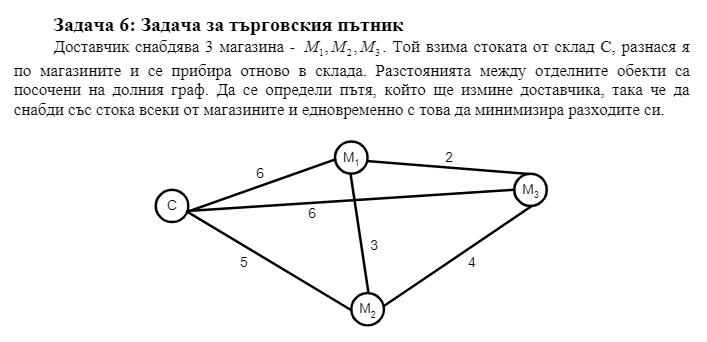
\includegraphics[width = \linewidth]{Pics/Discrete math/ex8/ex8-task6.png}
\end{figure}
Решение: \\
Необходимо е доставчикът да опише т.нар Хамилтонов контур, т.е. тръгвайки от склада С да мине последователно през всеки от магазините само по веднъж и отново да се върне в склада. В случая броя нa върховете на неориентирания граф е $n=4$. Следователно максималният брой различни Хамилтонови контури е $\frac{(n-1)!}{2} = \frac{3!}{2} = 3$, защото:
\begin{enumerate}
\item Фиксира се даден връх за $N_1$.
\item От връх $N_1$ може да се отиде до $(n-1)$ - нови върха, всеки от които може да се означи с връх $N_2$
\item При фиксирани връхове $N_1$ и $N_2$ от връх $N_2$ може да се отиде до $(n-2)$ - нови върха, всеки от които може да се означи с връх $N_1$ и т.н.
\end{enumerate}
$\implies$ Общият брой Хамилтонови контури е $(n-1)!$ -, но всеки два от тях са еднакви, но с противоположна посока на обхождане $\implies$ бщият брой Хамилтонови контури е $\frac{(n-1)!}{2}$.\\
Решението на конкретната задача ще се визуализира чрез моделиране на възможните Хамилтонови контури, използвайки граф-дърво.\\
\begin{figure} [htp!]
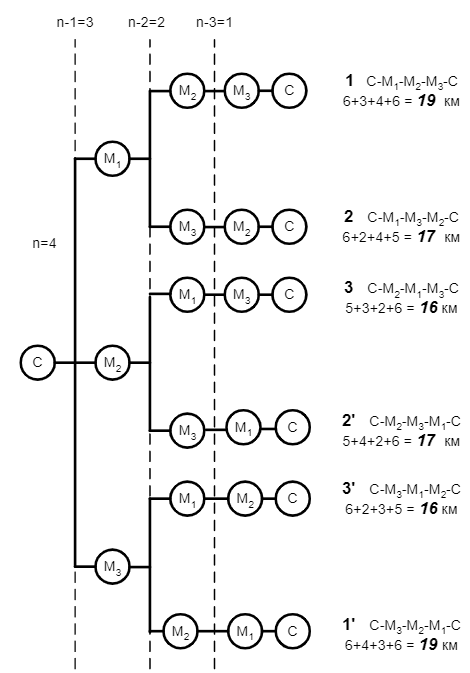
\includegraphics{Pics/Discrete math/ex8/ex8-task6-1.png}
\end{figure}
От дървото се вижда, че двойките контурите 1-1’,  2-2’ и 3-3’ са с равна дължина, но с обратна последователност на обхождане и най-краткият път е 3 (респ.3’),чиято дължина е 16км.

\subsubsection*{Задача 7}
\begin{figure} [htp!]
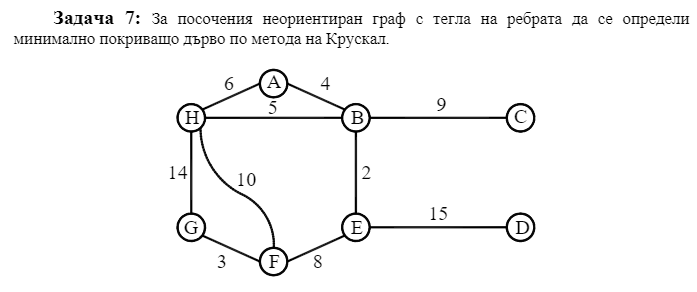
\includegraphics{Pics/Discrete math/ex8/ex8-task7.png}
\end{figure}
Последователността на присвояване на ребра на графа към МПД, съгласно алгоритъма на Крускал е следната: (B, E), (G, F), (A, B), (H,B), (F,E), (B,C), (E,D). \\
Резултантното МПД е показано на следващата фигура:
\begin{figure} [htp!]
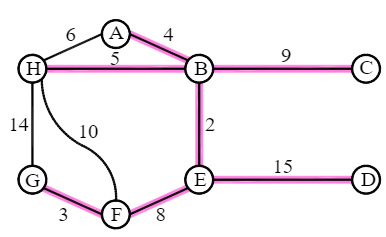
\includegraphics{Pics/Discrete math/ex8/ex8-task7-1.png}
\end{figure}
Съответстващата сума от тегловни коефициентина принадлежащите му ребра, е:
$$ 2 + 3 + 4 + 5 + 8 + 9 + 15 = 46$$
\newpage
\subsubsection*{Задача 8}
\begin{figure} [htp!]
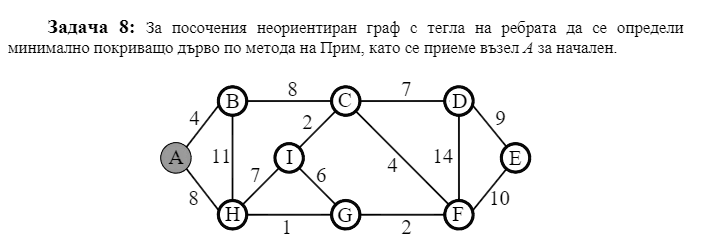
\includegraphics{Pics/Discrete math/ex8/ex8-task8.png}
\end{figure}
\begin{figure} [htp!]
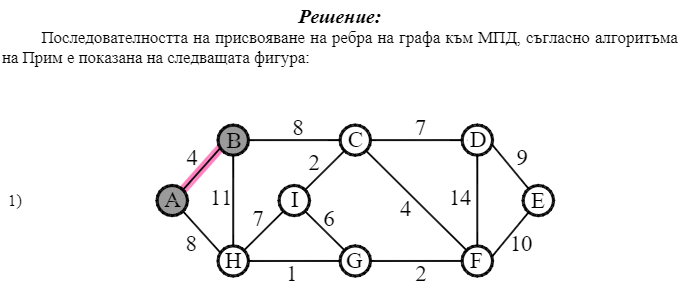
\includegraphics{Pics/Discrete math/ex8/ex8-task8-1.png}
\end{figure}
\begin{figure} [htp!]
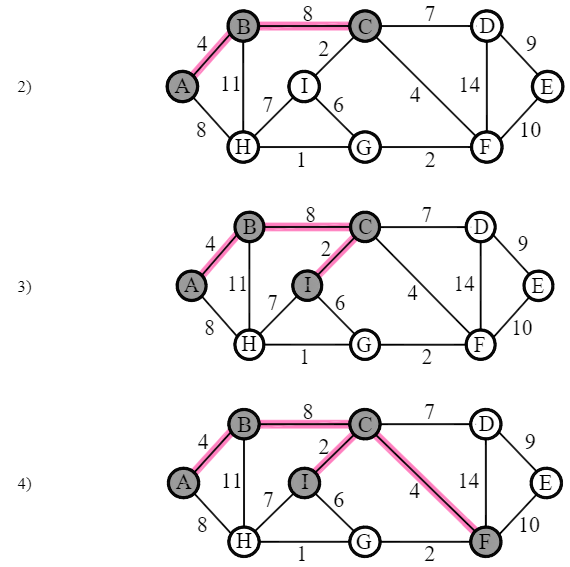
\includegraphics{Pics/Discrete math/ex8/ex8-task8-2.png}
\end{figure}
\begin{figure} [htp!]
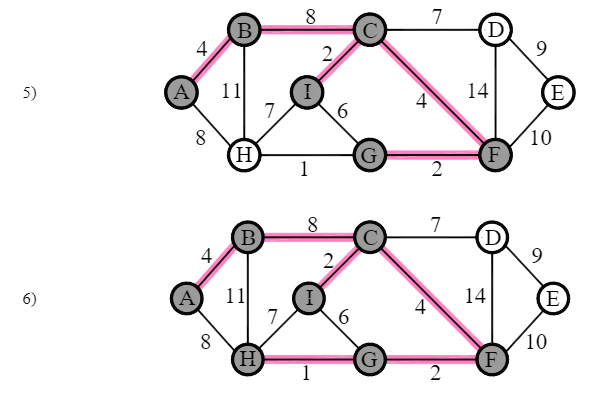
\includegraphics{Pics/Discrete math/ex8/ex8-task8-3.png}
\end{figure}
\begin{figure} [htp!]
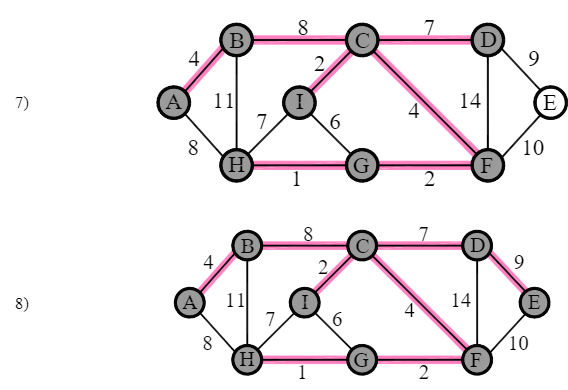
\includegraphics{Pics/Discrete math/ex8/ex8-task8-4.png}
\end{figure}
Съответстващата сума от тегловни коефициентина принадлежащите му ребра, е:
$$ 4 + 8 + 2 + 4 + 2 + 1 + 7 + 9 = 37$$
\newpage
\subsection{Упражнение 9}

\newpage
\subsection{ Упражнение 10}

\newpage
\subsection{ Упражнение 11}

\newpage
\subsection{ Упражнение 12}

\newpage
\subsection{ Упражнение 13}
























\end{document}